\subsection{The Fano mirror: a sub wavelength grating}\label{sec:fano_mirror}

\subsubsection{Geometric optical analysis}

Considering an ideal grating with period \emph{d} in the sub-wavelength regime, it can be shown that only a single mode of reflection/transmission is supported. 

Any grating, of arbitrary dimensions, must comply with the very general \emph{grating equation}\cite{Pedrotti} given as
\begin{equation}
    \sin \theta_m = m \frac{\lambda}{d},
\end{equation}
for the special case of a linearly polarized plane wave incident on a grating placed normal to the direction of propagation. Now, inserting the sub-wavelength condition \emph{d << $\lambda$}, it is easily seen that the right side of the equation blows up for any order of reflection $|m| > 0$, effectively showing that this is the aforementioned single supported mode in this regime. Furthermore, it can be equally easily seen that the propagation direction of the 0'th order mode is the same as the incident beam, i.e. normal to the grating.

\subsubsection{Reflection/transmission spectra and line shape analysis}

\subsubsection{Lossless grating}

We wish to analytically describe the wavelength-dependent spectra for the transmission and reflectivity of an infinite sub-wavelength grating. By first considering the case where absorption and thermal coupling effects are neglected, i.e. a lossless grating, we can assume conservation of energy and thereby the relations
\begin{equation}
    |r_g|^2+|t_g|^2=1 \hspace{0.5cm} \text{and} \hspace{0.5cm} |r_d|^2+|t_d|^2=1,
    \label{eq:energy conservation}
\end{equation}
where the subscripts \emph{g} and \emph{d} indicate the \emph{grating} and \emph{direct} transmissions and reflectivities, respectively. It is implied that the direct coefficients are constants and describe the transmission and reflectivity when the incident wavelength is significantly detuned from any guided-mode resonance of the grating. Furthermore, it is also implied that the grating coefficients are functions of the incident wavelength.

We now assume a normal incident beam on the grating as a linearly polarized monochromatic plane wave, with a wavelength close to a guided-mode resonance of the grating. In order to describe the coefficients $r_g$ and $t_g$ we follow the formalism presented by Fan and Joannopoulos \cite{Fan-Joannopoulos-guided-mode-resonance} and consider the likely paths of the incident light through the grating. It is quite intuitive to consider the case where the light is simply transmitted, and this shall be our first case hereafter denoted the \emph{direct pathway}. Another case one might consider is the one where the incident light excites the guided-mode resonance in the grating. This case is denoted the \emph{indirect pathway} and decays more slowly than it's direct counterpart. 

The interference caused when the guided mode is excited is often referred to as \emph{Fano resonances}, due to its physical similarities to the description of interference between a discrete autoionized state and a bound continuum state first reported by Fano \cite{Fano-theory}. The cross section of inelastic scattering, when measured as a function of energy, showed characteristic asymmetric peaks. These were described as the aforementioned interference pattern between \emph{direct} (the discrete state) and \emph{indirect} (the continuum state) pathways. 

By generalizing the model of Fan and Joannopoulos \cite{Fan-Joannopoulos-guided-mode-resonance} we describe the transmission and recletivity coefficent amplitudes as 
\begin{equation}
    r_g = r_d + \frac{a}{k-k_1 + i\gamma} \hspace{0.5cm} \text{and} \hspace{0.5cm} t_g = t_d + \frac{b}{k-k_1+i\gamma},
    \label{eq:ref/trans}
\end{equation}
where $k=2\pi/\lambda$ is the incident wave number, $k_1 = 2\pi/\lambda_1$ is the wave number according to the guided-mode resonance and $\gamma$ is the HWHM (half width at half maximum) of the guided-mode resonance. Complex coefficients $a$ and $b$ describe the interference between the directly transmitted or reflected waves and the guided mode of the grating. 

Note that in eq. (\ref{eq:ref/trans}) the right side of the expression for each coefficient corresponds to the continuum state i.e. the indirect pathway, while the direct transmission and reflection coefficients take the role of the autoionized discrete state, i.e. the direct pathway\footnote{The general eigenvector of a state comprised of a super-position between a discrete state and a continuum, i.e. a state vector corresponding to a Fano resonance, is given as $\Psi_E = a\phi + \int dE^{\prime} b_{E^{\prime}} \psi_{E^{\prime}}$, given in eq. (2) in ref. \cite{Fano-theory}, where $a$ and $b_{E^{\prime}}$ describes the probability of either pathway.} \cite{Fano-theory}

As we are dealing with an ideal, lossless, grating, we assume coefficients $a$ and $b$ to be equal, meaning that we specifically assume vertical symmetry throughout the grating. By considering eq. (\ref{eq:energy conservation}) this in turn leads to 
\begin{equation}
    a = b = -i \gamma (t_d + r_d),
\end{equation}
which further yields an expression for the grating transmission amplitude coefficient on the form
\begin{equation}
    t_g = t_d \frac{k - k_0}{k - k_1 + i \gamma}.
    \label{eq:lossless transmission coefficient}
\end{equation}
Here, the newly introduced $k_0 = 2\pi/\lambda_0$ is the zero-transmission/unity-reflectivity wave number.

To generalize eq. (\ref{eq:lossless transmission coefficient}) to include non-unity reflectivity and non-zero transmission, we allow for $a \neq b$ meaning that the case of vertical asymmetry is included in the model. By assuming $r_d,t_d \in \mathbb{R}$, eq. (\ref{eq:energy conservation}) leads to the coupled differential equations
\begin{equation}
    \begin{split}
        &t_d x_a + r_d x_b = 0, \hspace{0.3cm} \text{and} \\
        &x_a^2 + y_a^2 + x_b^2 + y_b^2 + 2 t_d \gamma y_a + 2 r_d \gamma y_b = 0,
    \end{split}
    \label{eq:lossless couples diff. eqs.}
\end{equation}
where $\{x,y\}_{a,b}$ respectively denotes the real and imaginary parts of the coefficients $a$ and $b$. Solving eqs. (\ref{eq:lossless couples diff. eqs.}) leads to the correct complex reflectivity coefficients and the expression for the transmission coefficient amplitudes now reads
\begin{equation}
    t_g = t_d \frac{k - k_0 + i \beta}{k - k_1 + i \gamma},
    \label{eq:lossy transmission coefficients}
\end{equation}
where $k_0$ and $\beta$ are defined from the expression for $a$ found by solving eqs. (\ref{eq:lossless couples diff. eqs.}), given as
\begin{equation}
    a = t_d (k_1 - k_0 - i \gamma + i \beta).
\end{equation}
Finally, this allows for non-zero transmission and non-unity reflectivity at wave number $k_0$.

\begin{figure}[h!]
    \centering
    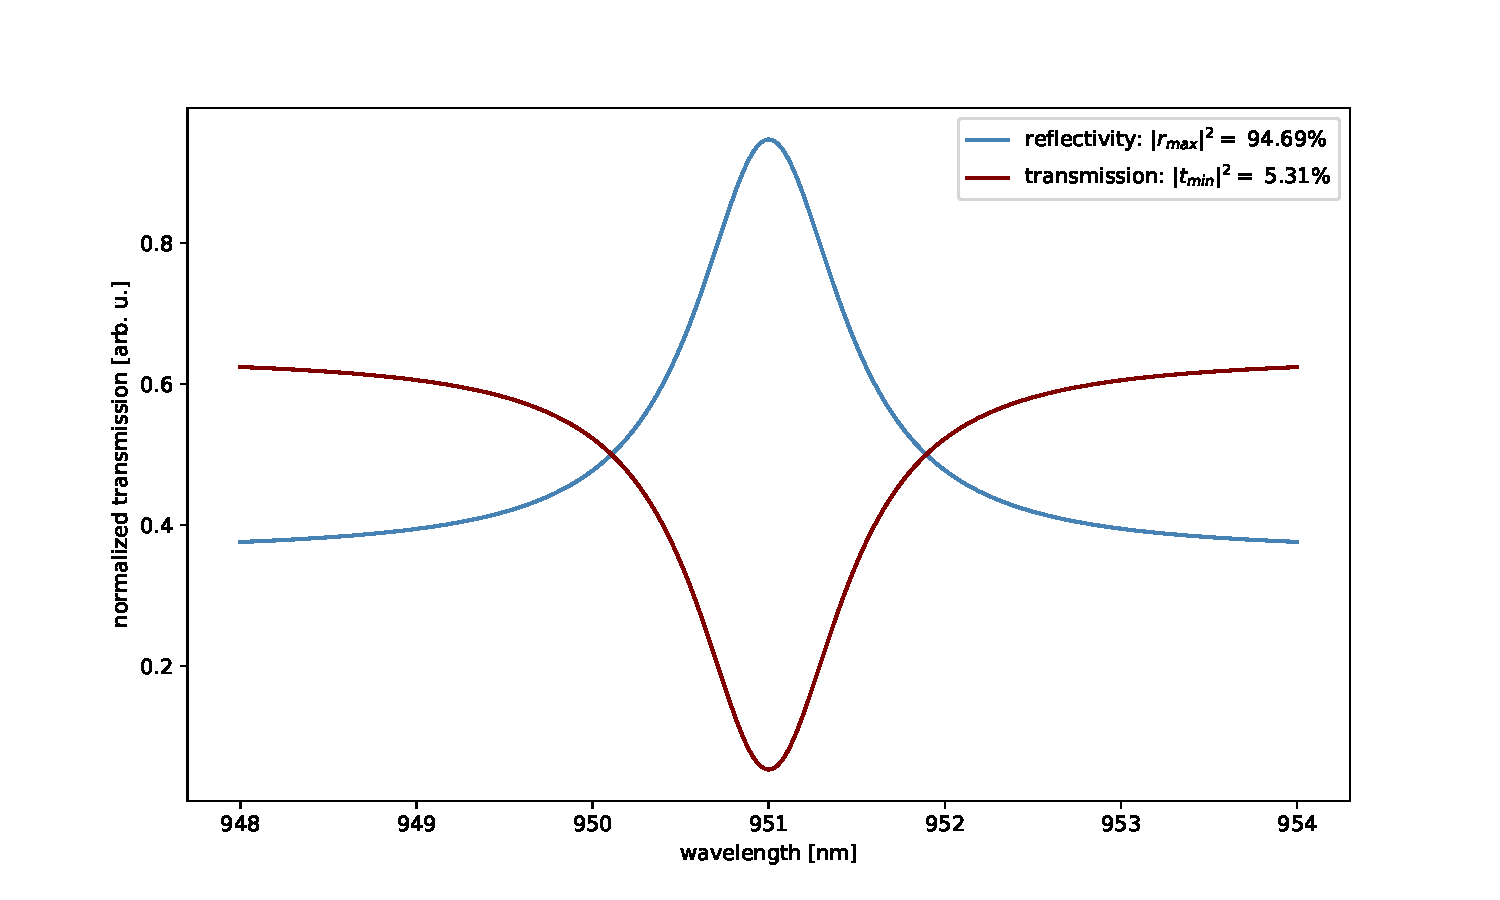
\includegraphics[width=0.6\textwidth]{figures/grating_spectrum_lossless_example.pdf}
    \caption{Simulated reflectiviy and transmission spectra of an arbitrary lossless grating.}
    \label{fig:lossless_grating_spectrum}
\end{figure}

\subsubsection{Lossy grating}

In order to modify the above model such that losses, e.g. due to absorption or thermal coupling effects, are accounted for, we add a resonant loss term to the energy conservation relation in eq. (\ref{eq:energy conservation}). For this we introduce the resonant loss level $L$, which must be known in order to accurately calculate the complex reflectivity coefficients. The energy conservation relation is modified such that
\begin{equation}
    |t_g|^2 + |r_g|^2 + \frac{c^2}{(k - k_1)^2 + \gamma^2} = 1,
    \label{eq:lossy energy conservation}
\end{equation}
where the coefficient $c^2 = L((k-k_1)^2 + \gamma^2)$ includes the resonant loss term $L$. A new set of coupled differential equations are found, using eq. (\ref{eq:lossy energy conservation}), given as
\begin{equation}
    \begin{split}
        &t_d x_a + r_d x_b = 0, \hspace{0.3cm} \text{and} \\
        &x_a^2 + y_a^2 + x_b^2 + y_b^2 + c^2 +  2 t_d \gamma y_a + 2 r_d \gamma y_b = 0.
    \end{split}
    \label{eq:lossy couples diff. eqs.}
\end{equation}
It is easily identified that eq. (\ref{eq:lossless couples diff. eqs.}) and eq. (\ref{eq:lossy couples diff. eqs.}) differ only by the addition of coefficient $c^2$, and thereby the losses. Solving eq. (\ref{eq:lossy couples diff. eqs.}) leads to the correct complex reflectivity coefficients, except that they now account for any losses associated with the grating. 

In conclusion, the complete grating model consists of an expression for the transmission coefficients and a set of coupled differential equations for the reflection coefficients, shown in eq. (\ref{eq:lossy transmission coefficients}) and eq. (\ref{eq:lossy couples diff. eqs.}), respectively. The model on the form used for this project and subsequent thesis is derived in previous work by A. Darki et al. \cite{Darki} and more recently T. Mitra et al. \cite{Mitra}.

\begin{figure}[h!]
    \centering
    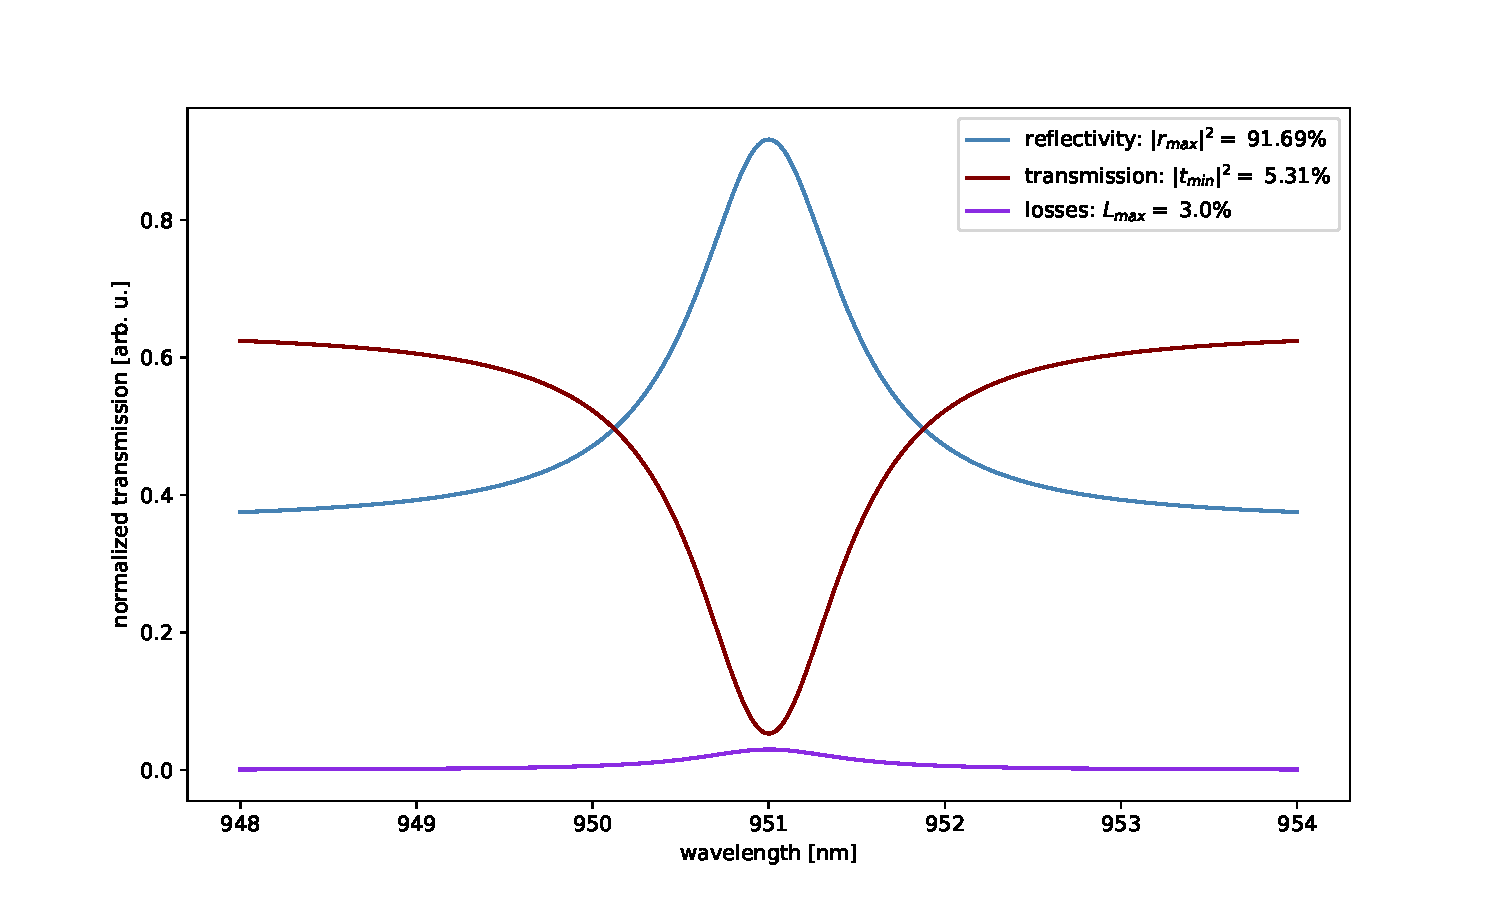
\includegraphics[width=0.6\textwidth]{figures/grating_spectrum_lossy_example.pdf}
    \caption{Simulated reflectiviy and transmission spectra of an arbitrary lossy grating.}
    \label{fig:lossy_grating_spectrum}
\end{figure}

\subsection{The Fano cavity}

\subsubsection{The single Fano cavity model}

The single Fano cavity consists of a planer broadband mirror, and a sub-wavelength grating, i.e. a Fano mirror, as described in section \ref{sec:fano_mirror} and seen in figure \ref{fig:broadband_and_single_fano_sketch} where schematics of the single Fano and broadband cavity configurations are shown. While the broadband mirror has fixed optical properties, the Fano mirror has transmission and reflection coefficients dependent on the incident wavelength, according to solutions to the doupled differential equations of eq. (\ref{eq:lossy couples diff. eqs.}). 

\begin{figure}[h!]
    \centering
    \begin{subfigure}[b]{0.3\textwidth}
        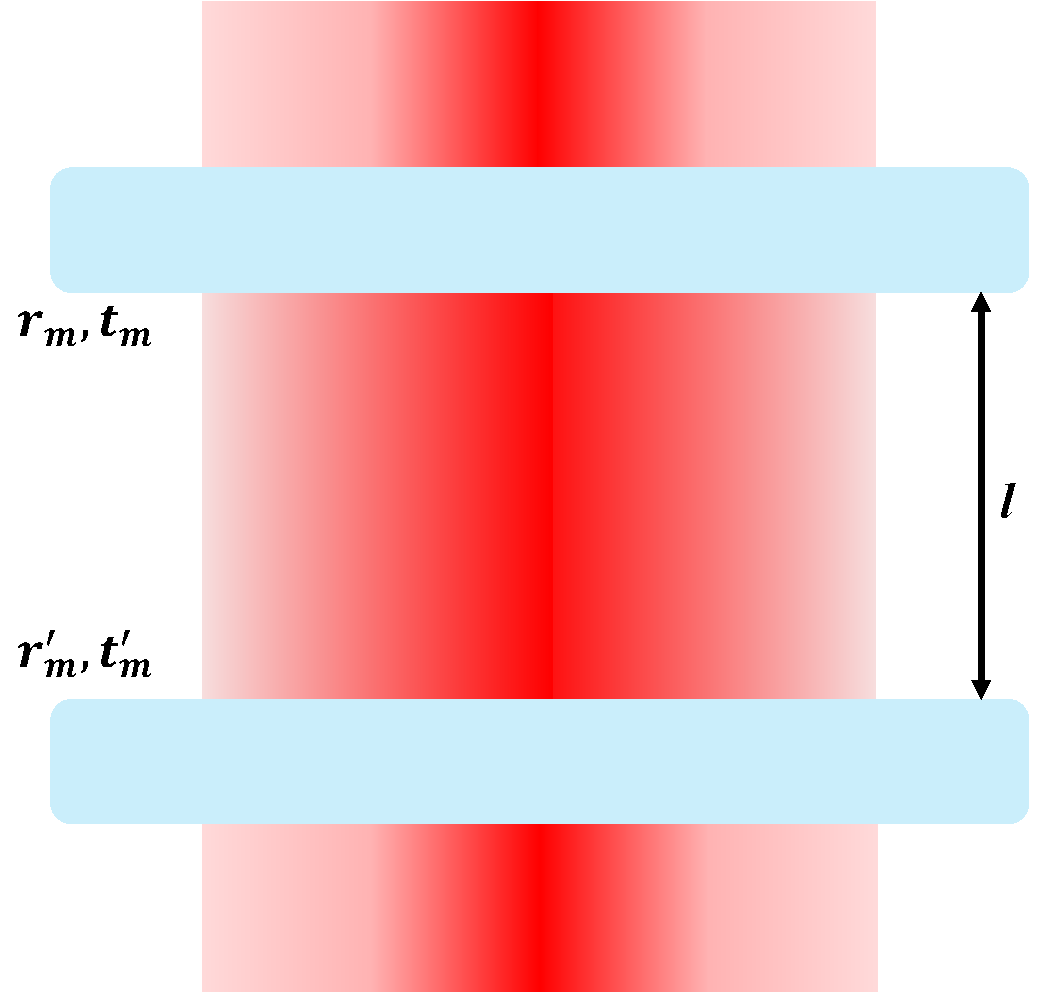
\includegraphics[width=\textwidth]{figures/broadband_sketch.pdf}
        \caption{Schematics of the broadband cavity.}
        \label{fig:broadband_sketch}
    \end{subfigure}
    \hspace{1cm}
    \begin{subfigure}[b]{0.3\textwidth}
        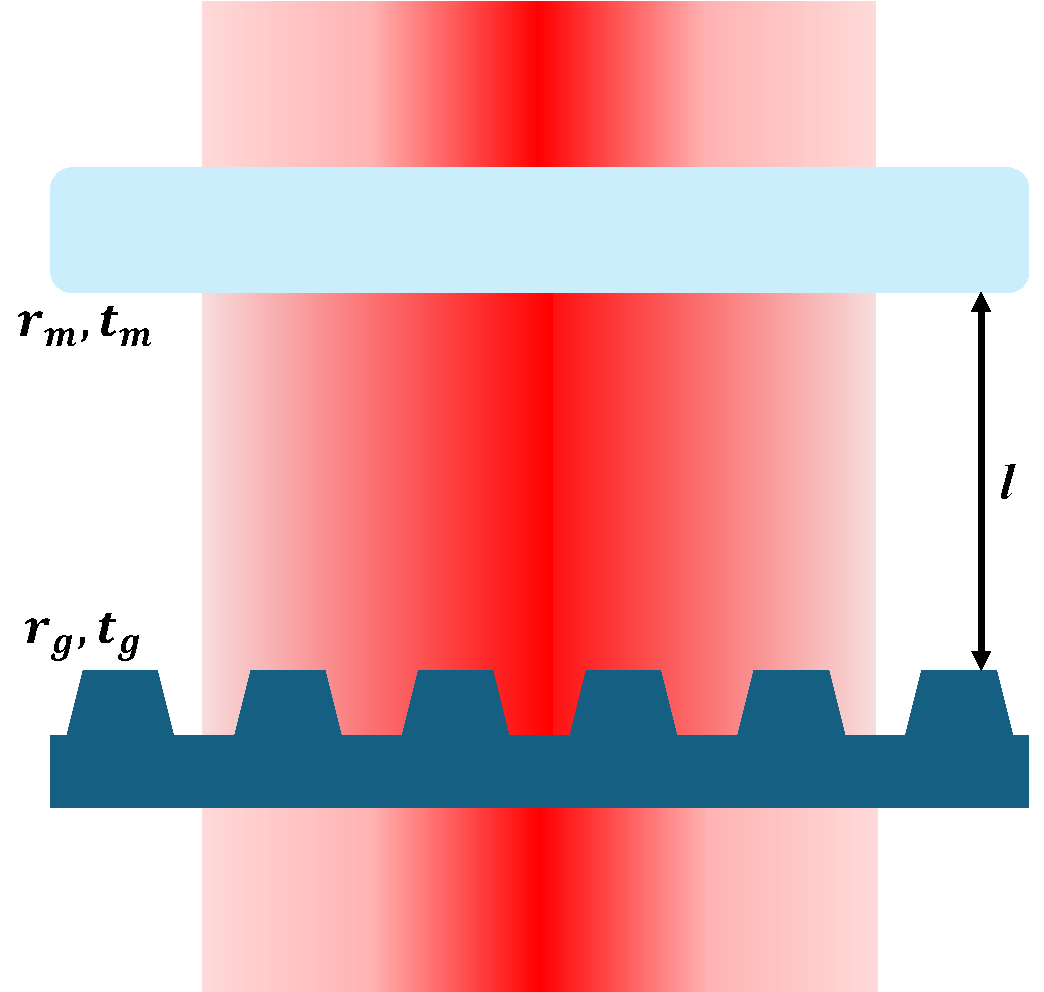
\includegraphics[width=\textwidth]{figures/single_fano_sketch.pdf}
        \caption{Schematics of the single Fano cavity.}
        \label{fig:single_fano_sketch}
    \end{subfigure}
    \caption{}
    \label{fig:broadband_and_single_fano_sketch}
\end{figure}

In order to model the single Fano cavity transmission spectra, we therefore consider the transmission function of a normal incident and planer Fabry-Perot cavity in eq. (\ref{eq:fabry_perot_trans}) with $r,t \rightarrow r_m,t_m$ and $r^{\prime},t^{\prime} \rightarrow r_g(\lambda),t_g(\lambda)$. Here the subscript $m$ indicates the broadband \emph{mirror} coefficients, and $g$ is for \emph{grating}, which indicates the coefficients of the Fano mirror. Rewriting eq. (\ref{eq:fabry_perot_trans}) such that it describes the normalized transmission amplitude, through the single Fano cavity, $T_{cav} = |E_{out}|^2/|E_{0,in}|^2$ we get
\begin{equation}
    T_{cav} = \left|\frac{t_m t_g(\lambda) e^{i\phi}}{1 - r_m r_g e^{2i\phi}}\right|^2,
    \label{eq:single_fano_trans}
\end{equation}
where $\phi = 2\delta = kl$, $k=2 \pi / \lambda$ and $l$ is the cavity length, as is consistent the general case described in section \ref{sec:fano_mirror}.

\subsubsection{Transmission linewidth}\label{sec:single_fano_cavity_trans_linewidth}

In order to analytically describe how the transmission spectrum at, or close to, overall resonance\footnote{This terminology is used for the scenario where the guided-mode, cavity mode and input laser mode all meet the resonance condition $\lambda_g \approx \lambda_c \approx \lambda_l$, where $g,c,l$ stands for grating/guided-mode, cavity and laser, respectively.} behaves as a function of the incident wavelength, we attempt to generalize the Fano model for this specific regime. Considering the case where the cavity resonance closely resembles the guided-mode resonance of the Fano mirror (the zero-transmission wavelength), eq. (\ref{eq:single_fano_trans}) can be approximated well by
\begin{equation}
    T_{cav} \approx \frac{A}{1 + \left( \frac{\Delta}{1 - \nu \Delta} \right)^2},
    \label{eq:general_fano_model}
\end{equation}
where $\Delta = (\lambda - \lambda_c) / \delta \lambda$ is the detuning from the cavity resonance normalized by the HWHM $\delta \lambda$, and $\nu$ is a constant describing the asymmetry of the single Fano transmission spectrum. 

From eq. (\ref{eq:general_fano_model}) it can be shown that the HWHM of the Fano transmission profile around the resonance wavelength $\delta \lambda$ is approximately given as
\begin{equation}
    \delta \lambda \approx \frac{1}{\frac{1}{\delta \lambda_c} + \frac{1}{\delta \lambda_g}},
    \label{eq:analytical_linewidth}
\end{equation}
where $\delta \lambda_c$, $\delta \lambda_g$ are the contributions to the linewidth stemming from the broadband cavity and the Fano cavity in the Fano regime, respectively. It can be shown that there are two regimes of interest when examining the linewidth of the Fano cavity transmission profile. The first of these is the standard cavity regime, where the broadband and Fano cavity produces resonance transmission peaks of comparable, if not equal, linewidths. The other is the aforementioned Fano regime where a significant reduction in linewidth is found, when comparing the Fano and broadband cavity transmission profiles. In order to detemine where the transition between the standard and the Fano cavity regimes occur, we look at the expressions for $\delta \lambda_c$ and $\delta \lambda_g$ included in eq. (\ref{eq:analytical_linewidth}). The standard cavity linewidth is given as
\begin{equation}
    \delta \lambda_c = \frac{\lambda_0^2}{8 \pi l} (|t_g(\lambda_0)|^2 + |t_m|^2 + L),
    \label{eq:analytical_linewidth_broadband}
\end{equation}
while the Fano cavity linewidth in the Fano regime is given as
\begin{equation}
    \delta \lambda_g = \frac{\gamma \lambda}{2 (1-r_d)}(|t_g(\lambda_0)|^2 + |t_m|^2 + L).
\end{equation}
Here $\lambda_0$ is the cavity resonance wavelength, $l$ is the cavity length, $L = 1 - |r_g(\lambda_0)|^2$ is the total losses of the cavity when on resonance, $\gamma \lambda$ is the width of the guided-mode resonance of the Fano mirror and $r_d$ is the off-resonance, or \emph{direct}, reflectivity of the Fano mirror.

\begin{figure}[h!]
    \centering
    \begin{subfigure}[b]{0.49\textwidth}
        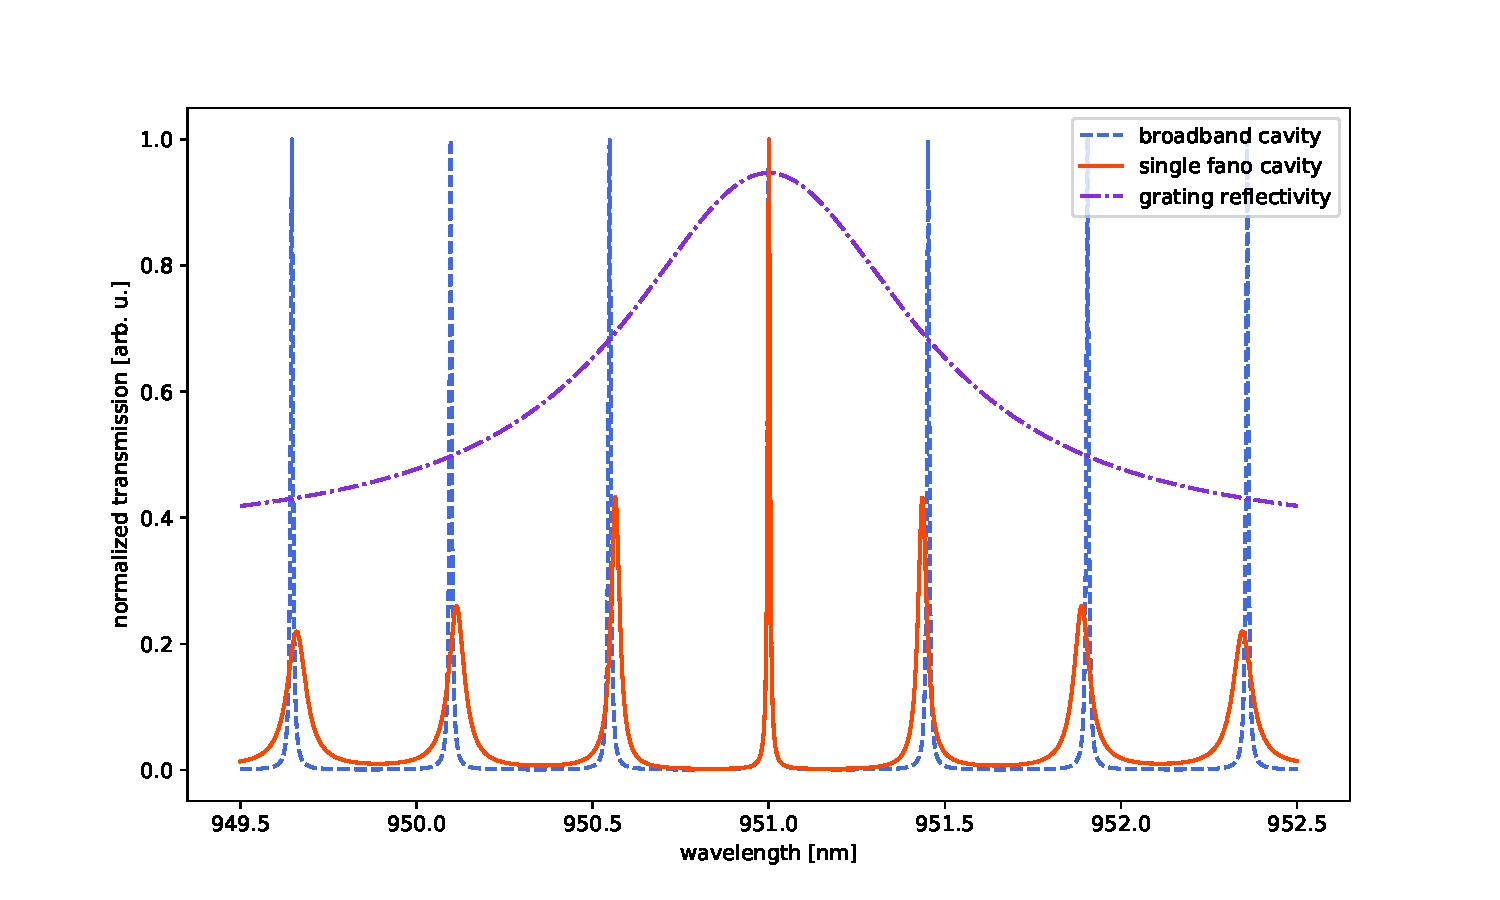
\includegraphics[width=\textwidth]{figures/fano_and_broadband_cavity_1000um.pdf}
        \caption{Broadband and single Fano transmissions for a cavity length of $\sim 1000 \mu m$, i.e. in the \emph{standard} regime.}
        \label{fig:standard_regime_trans}
    \end{subfigure}
    \begin{subfigure}[b]{0.49\textwidth}
        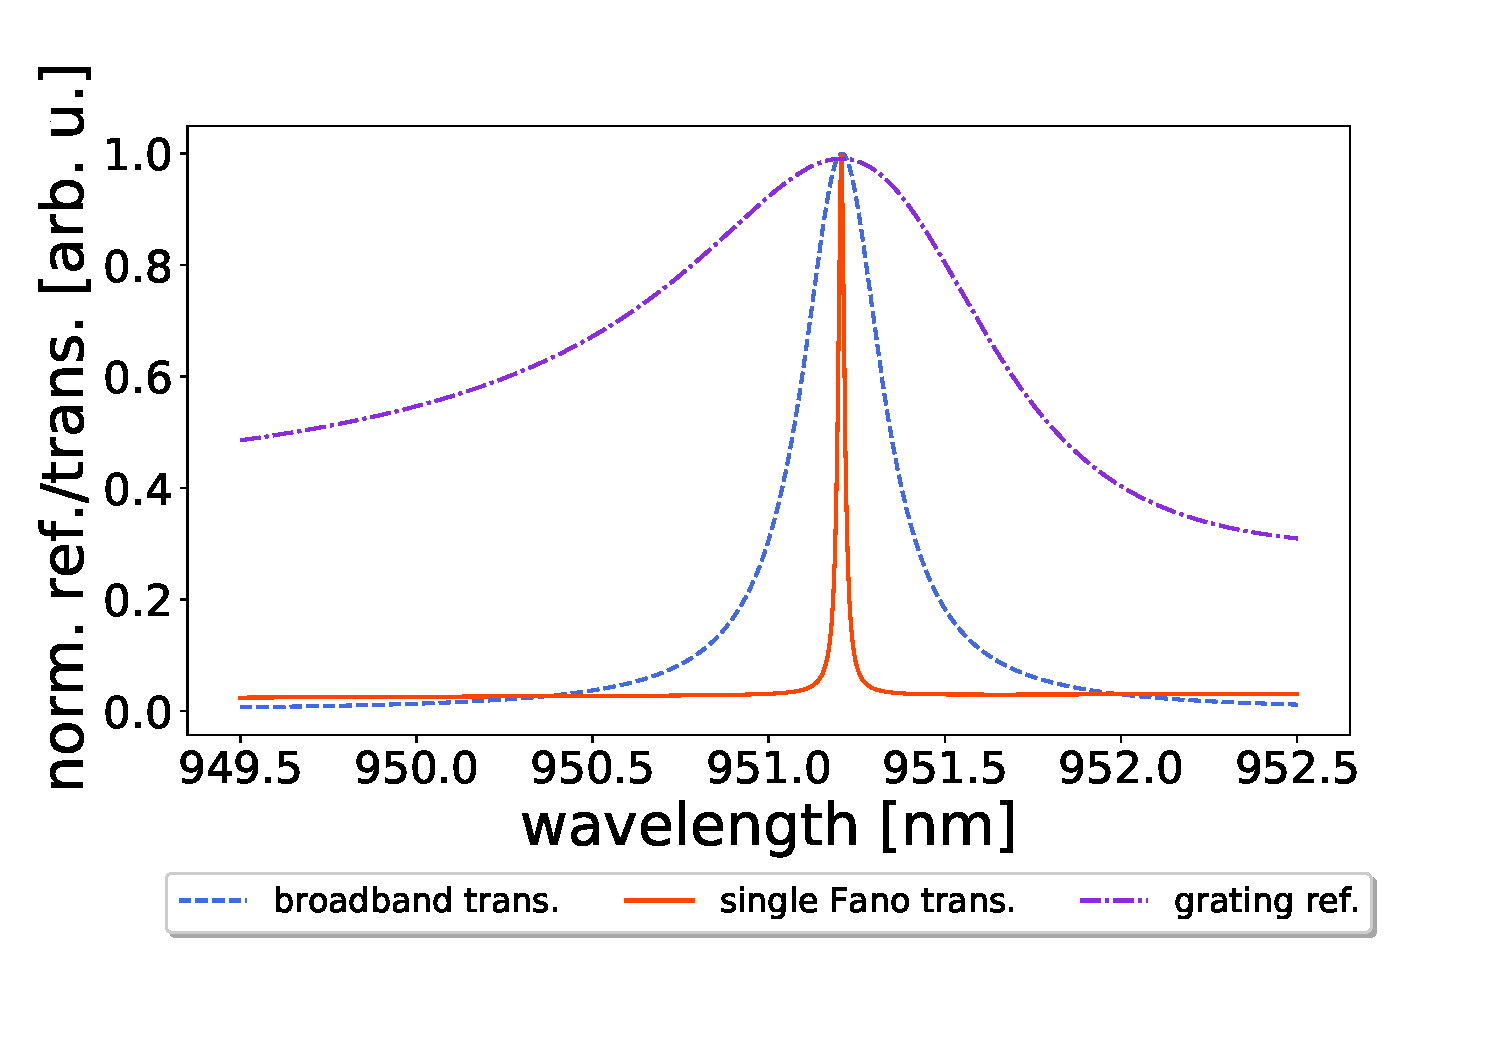
\includegraphics[width=\textwidth]{figures/fano_and_broadband_cavity_5um.pdf}
        \caption{Broadband and single Fano transmissions for a cavity length of $\sim 5 \mu m$, i.e. in the \emph{Fano} regime.}
        \label{fig:fano_regime_trans}
    \end{subfigure}
\end{figure}

Figures \ref{fig:standard_regime_trans} and \ref{fig:fano_regime_trans} depicts two examples of single Fano cavity transmission spectra together with their respective complimentary broadband cavity transmission profiles, and the reflectiviy amplitude of the Fano mirror used to model both profiles. As shown in section \ref{sec:fano_mirror} any Fano mirror, or grating, is described by five characterizing parameters. For the one used to model the transmission spectra in figures \ref{fig:standard_regime_trans} and \ref{fig:fano_regime_trans}  these are 
\begin{equation}
    \begin{split}
    \lambda_0 = &951 nm,\:\: \lambda_1 = 951 nm,\:\: t_d = 80\%,\\ &\gamma \lambda = 0.5 nm\: \text{ and }\: \beta = 10^{-6},
    \end{split}
\end{equation}
where we remember that $\lambda_{0,1}$ are the resonant wavelengths for, respectively, the cavity and guided-mode, $t_d$ is the direct transmission, $\gamma \lambda$ is the width of the guided-mode resonance and $\beta$ is a constant describing the losses of the grating, which here is neglected when solving the coupled differential equantions of eq. (\ref{eq:lossy couples diff. eqs.}). The broadband mirror parameters are chosen such that it perfectly resembles the transmission and reflectivity of the grating on resonance, which is arbitrarily chosen such that $|r_{m}|^2=95\%$ and $|t_{m}|^2 = 5\%$.

It is clear from inspection of figure \ref{fig:standard_regime_trans} that the resonance transmission profile of the standard broadband cavity is not wavelength dependent, in the sense that all fringes, when cavity losses are neglected, appear to have the same high finesse $\mathcal{F}$, i.e. ratio between the FSR and HWHM. This is not the case for the Fano cavity which is, naturally, due to the wavelength dependence of the optical properties of the Fano mirror, as this causes the transmission and reflectivity to \emph{only} match those of the broadband mirror when on resonance. 

In figure \ref{fig:fano_regime_trans}, the transmission spectra of both cavities are shown \emph{in} the Fano regime, where it is clearly seen that while the standard cavity experiences broadening for shorter cavity lengths\footnote{This is a natural consequence of the shorter cavity as this causes the lifetime inside the cavity to fall and hense the transmission HWHM to rise. The HWHM is inversly proportional to the lifetime and goes as $\delta \lambda \propto 1/\tau$.}, this is not the case for the Fano cavity transmission peak.

\begin{figure}[h!]
    \centering
    \begin{subfigure}[c]{0.64\textwidth}
        \centering
        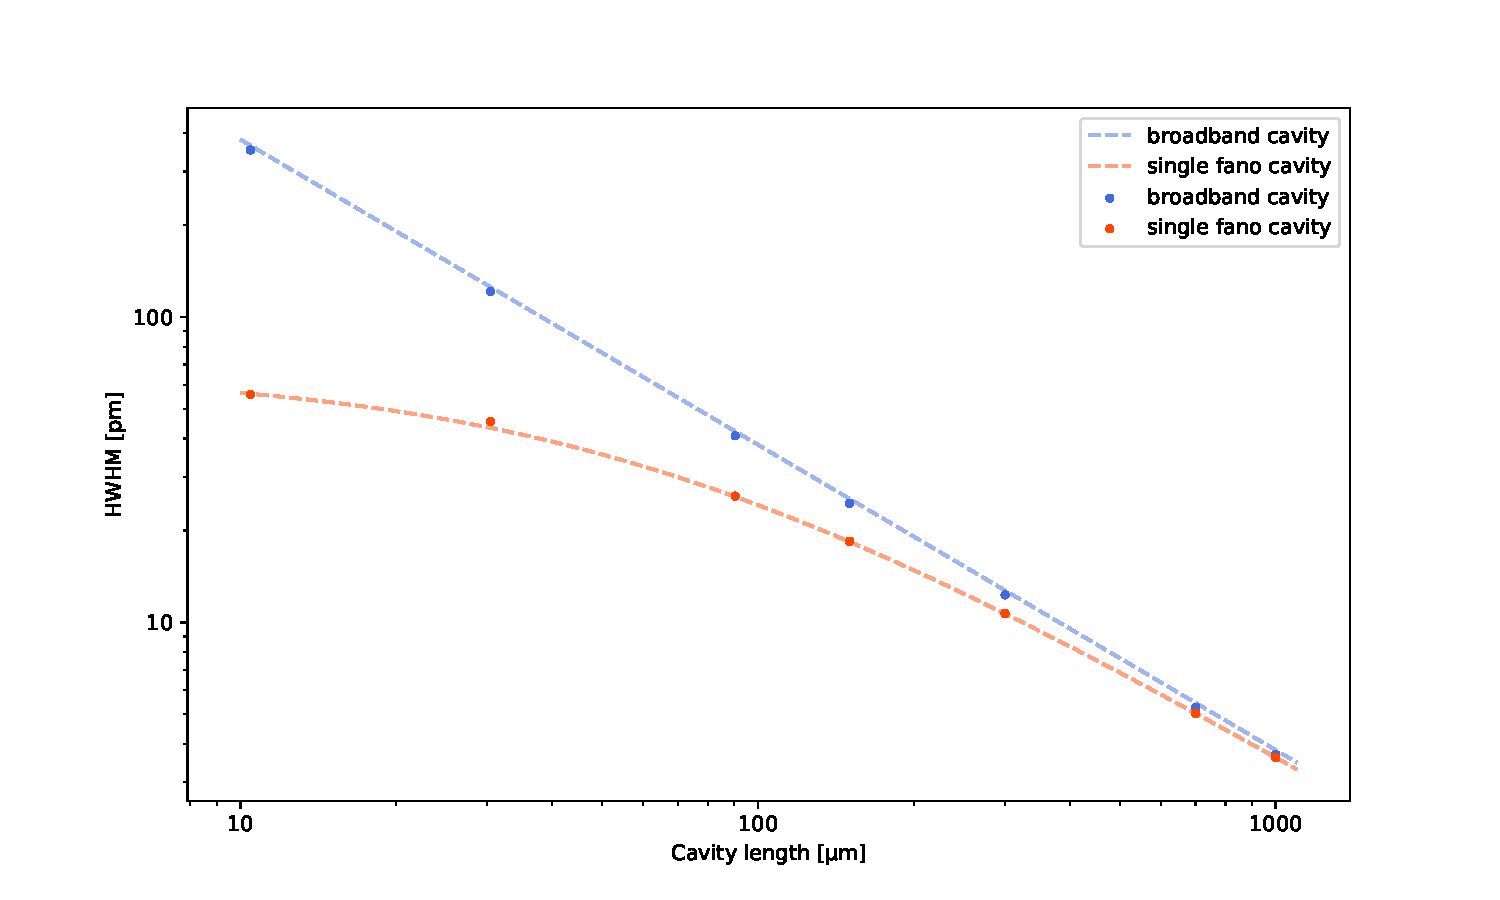
\includegraphics[width=\textwidth]{figures/HWHM_broadband_vs_single_sim.pdf}
        \caption{The approximate analytical resonance linewidths (eq. (\ref{eq:analytical_linewidth})) as a function of cavity length for the broadband and single Fano cavities are shown together with linewidths of transmission profiles simulated using eq. (\ref{eq:single_fano_trans}) and eq. (\ref{eq:fabry_perot_trans}) for comparison.}
        \label{fig:HWHM_broadband_vs_single_fano}
    \end{subfigure}
    \begin{subfigure}[c]{0.34\textwidth}
        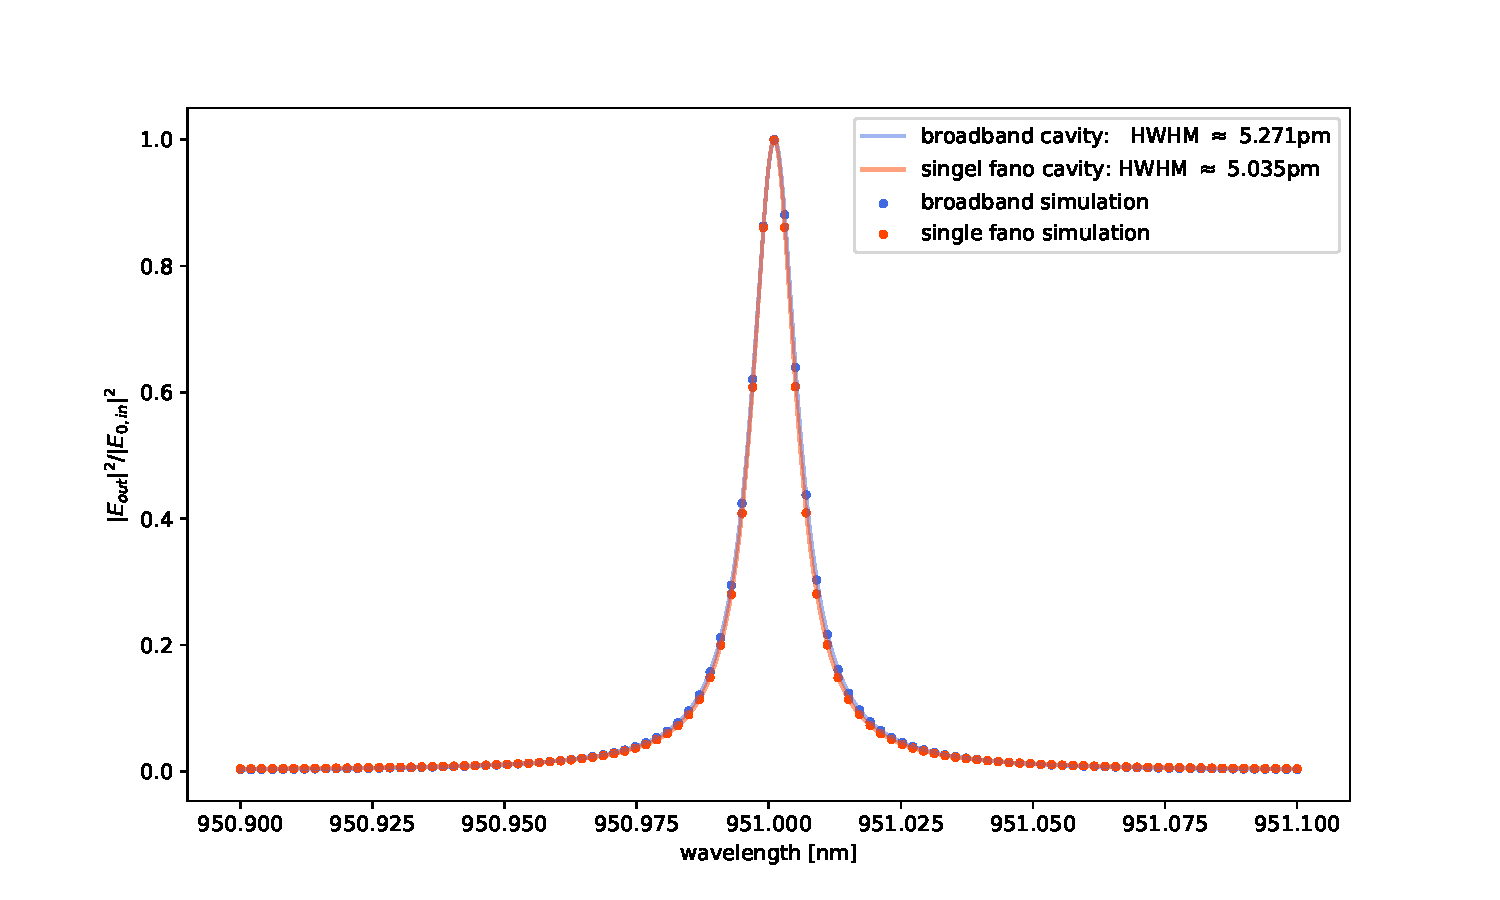
\includegraphics[width=\textwidth]{figures/sim_single_vs_broadband_700um.pdf}
        \caption{Transmission spectra of broadband and single Fano cavities of length $\sim 700 \mu m$.}
        \label{fig:700um_broadband_and_single_fano_peak}
        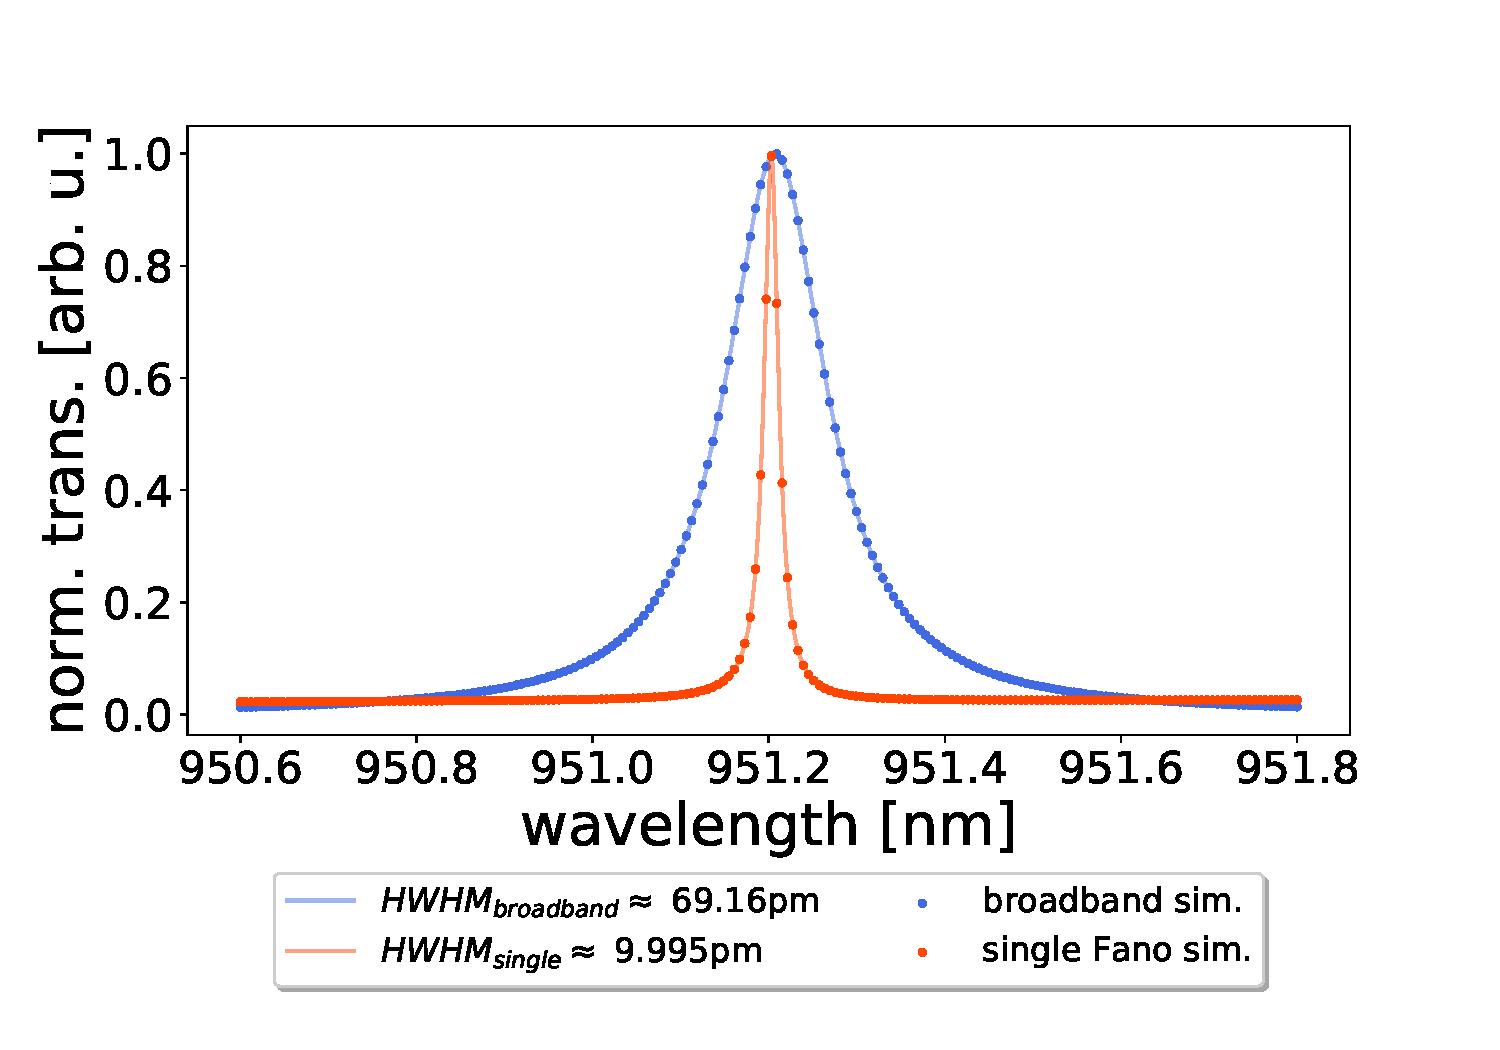
\includegraphics[width=\textwidth]{figures/sim_single_vs_broadband_10um.pdf}
        \caption{Transmission spectra of broadband and single Fano cavities of length $\sim 10 \mu m$.}
        \label{fig:10um_broadband_and_single_fano_peak}
    \end{subfigure}
\end{figure}

Figure \ref{fig:HWHM_broadband_vs_single_fano} models the behavior of the linewidth of the single Fano cavity compared with the one for a broadband cavity of similar optical properties, as a function of wavelength. Here it is easily seen where the linewidth of the single Fano begins to saturate, and hence deviate from the one of the broadband cavity. The plotted line in the figure is calculated using eq. (\ref{eq:analytical_linewidth}) while the points depicit linewidths found as a fitting parameter from a least squares fit of the general Fano model in eq. (\ref{eq:general_fano_model}) to transmission spectra simulated by the Fabry-Perot (eq. (\ref{eq:fabry_perot_trans})) and single Fano (eq. (\ref{eq:single_fano_trans})) transmission functions. Finally, it can be concluded that the approximate analytical expression for the linewidth of the broadband and single fano cavities in eq. (\ref{eq:analytical_linewidth}) correlates very well with the values found from the simulated spectra.

\subsection{The double Fano cavity}

\subsubsection{The double fano transmission model}

While the single Fano cavity is usually known in the appropriate litterature as simply a \emph{Fano cavity}, I have insisted on including the fact that it contains only one Fano mirror, and hence denoted it the \emph{single} Fano cavity. This addition is justified by the contents of this section, and namely that we now move on to the \emph{double} Fano cavity, which as the name suggests consists of two Fano mirrors. The schematics of this configuration is shown together with the one for the single Fano cavity in figure \ref{fig:single_and_double_fano_sketch}.

\begin{figure}[h!]
    \centering
    \begin{subfigure}[b]{0.3\textwidth}
        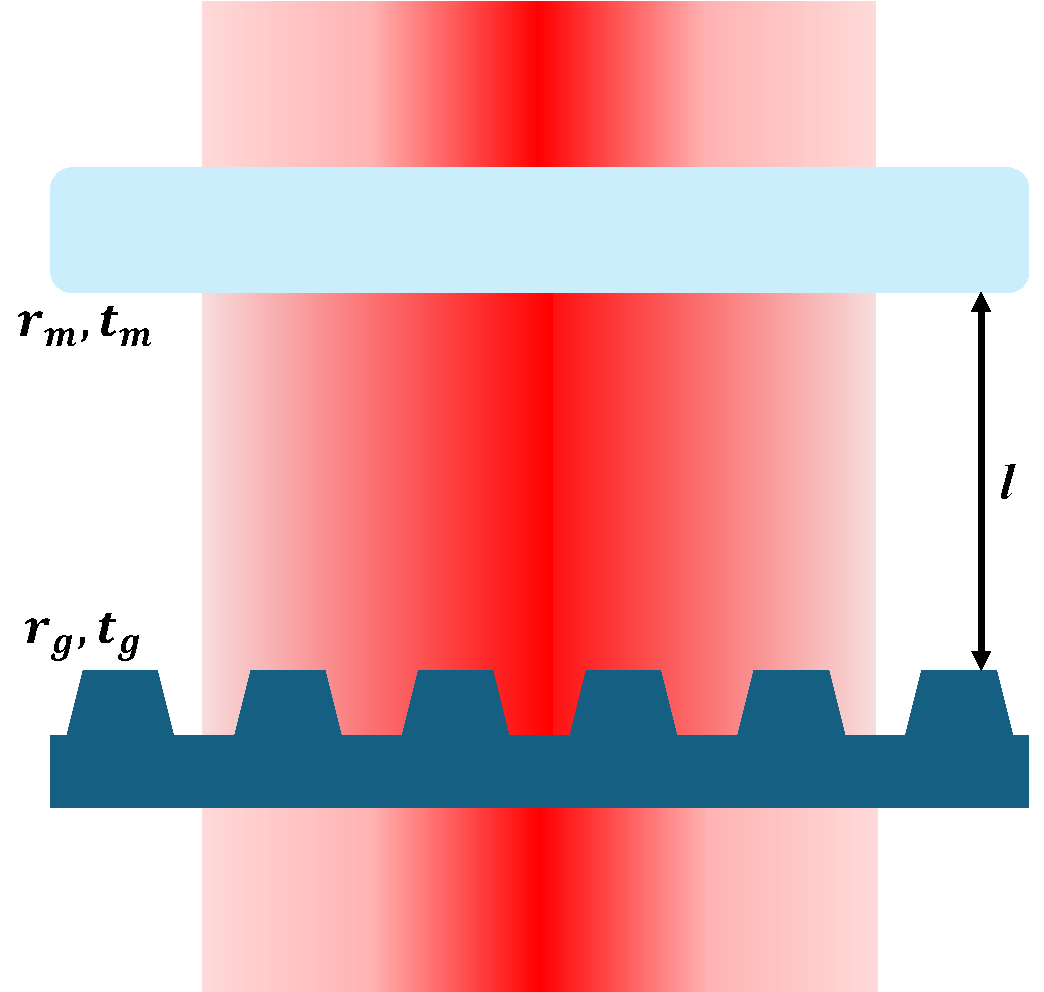
\includegraphics[width=\textwidth]{figures/single_fano_sketch.pdf}
        \caption{Schematics of the single Fano cavity.}
        \label{fig:single_fano_sketch2}
    \end{subfigure}
    \hspace{1cm}
    \begin{subfigure}[b]{0.3\textwidth}
        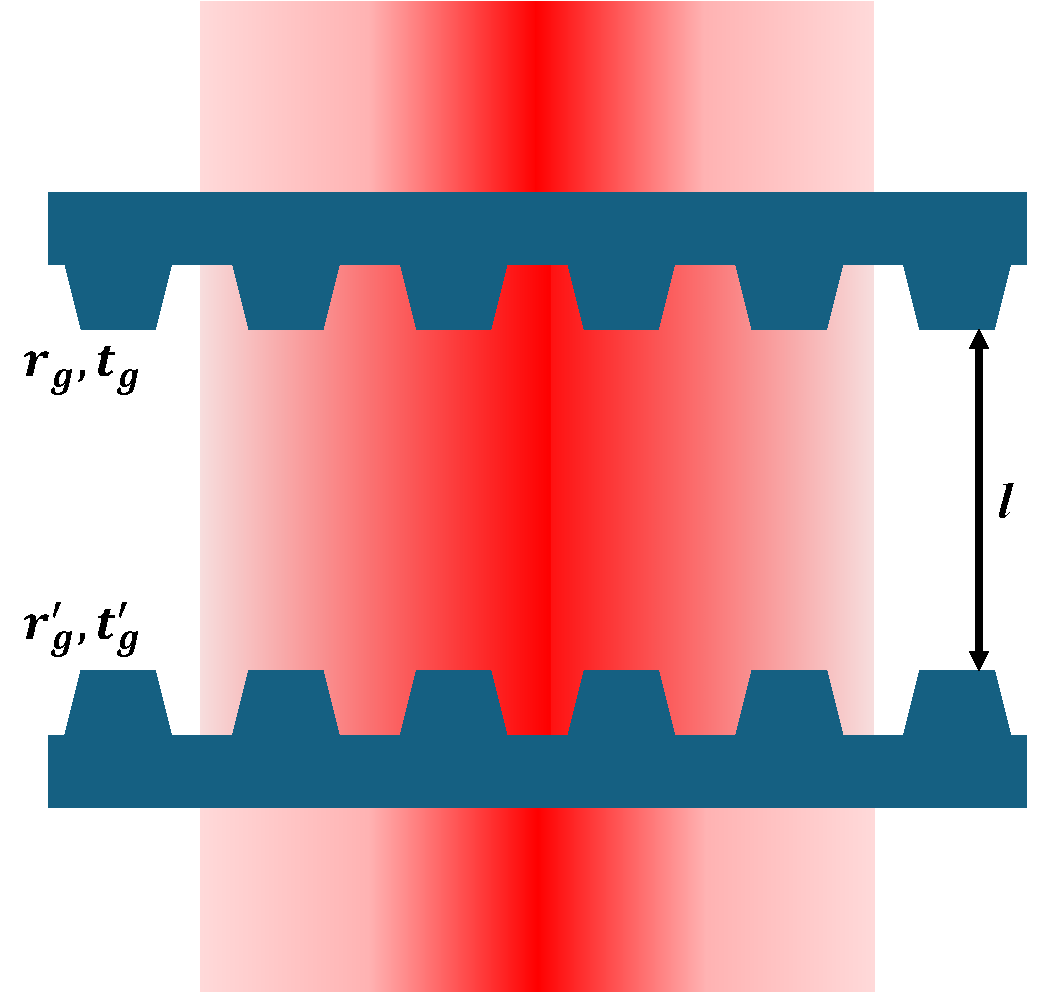
\includegraphics[width=\textwidth]{figures/double_fano_sketch.pdf}
        \caption{Schematics of the double Fano cavity.}
        \label{fig:double_fano_sketch}
    \end{subfigure}
    \caption{}
    \label{fig:single_and_double_fano_sketch}
\end{figure}

Here it is evident that instead of having one set of reflectivity and transmission coefficients that depend on the incident wavelength, we now have two. In order to model the transmission of the double Fano cavity, we once again consider the transmission function for the normal incident and planar Fabry-Perot cavity in eq. (\ref{eq:fabry_perot_trans}), this time with $r,t \rightarrow r_g(\lambda),t_g(\lambda)$ and $r^{\prime},t^{\prime} \rightarrow r_g^{\prime}(\lambda),t_g^{\prime}(\lambda)$. We rewrite the Fabry-Perot transmission function with the addressed substitutions of the optical coefficients and such that it decribes the normalized transmission amplitudes $T_{cav} = |E_{out}|^2/|E_{0,in}|^2$ and get
\begin{equation}
    T_{cav} = \frac{t_g(\lambda) t_g^{\prime}(\lambda) e^{i\phi}}{1 - r_g(\lambda)r_g^{\prime}(\lambda) e^{2 i \phi}}.
    \label{eq:double_fano_transmission}
\end{equation}
The subscript $g$ indicates a grating transmission or reflectivity. Figure \ref{fig:double_fano_transmission} shows an example of the normalized transmission spectrum of an $\sim 30 \mu m$ double Fano cavity on- and off-resonance, found using eq. (\ref{eq:double_fano_transmission}).

\begin{figure}[h!]
    \centering
    \begin{subfigure}[c]{0.49\textwidth}
        \centering
        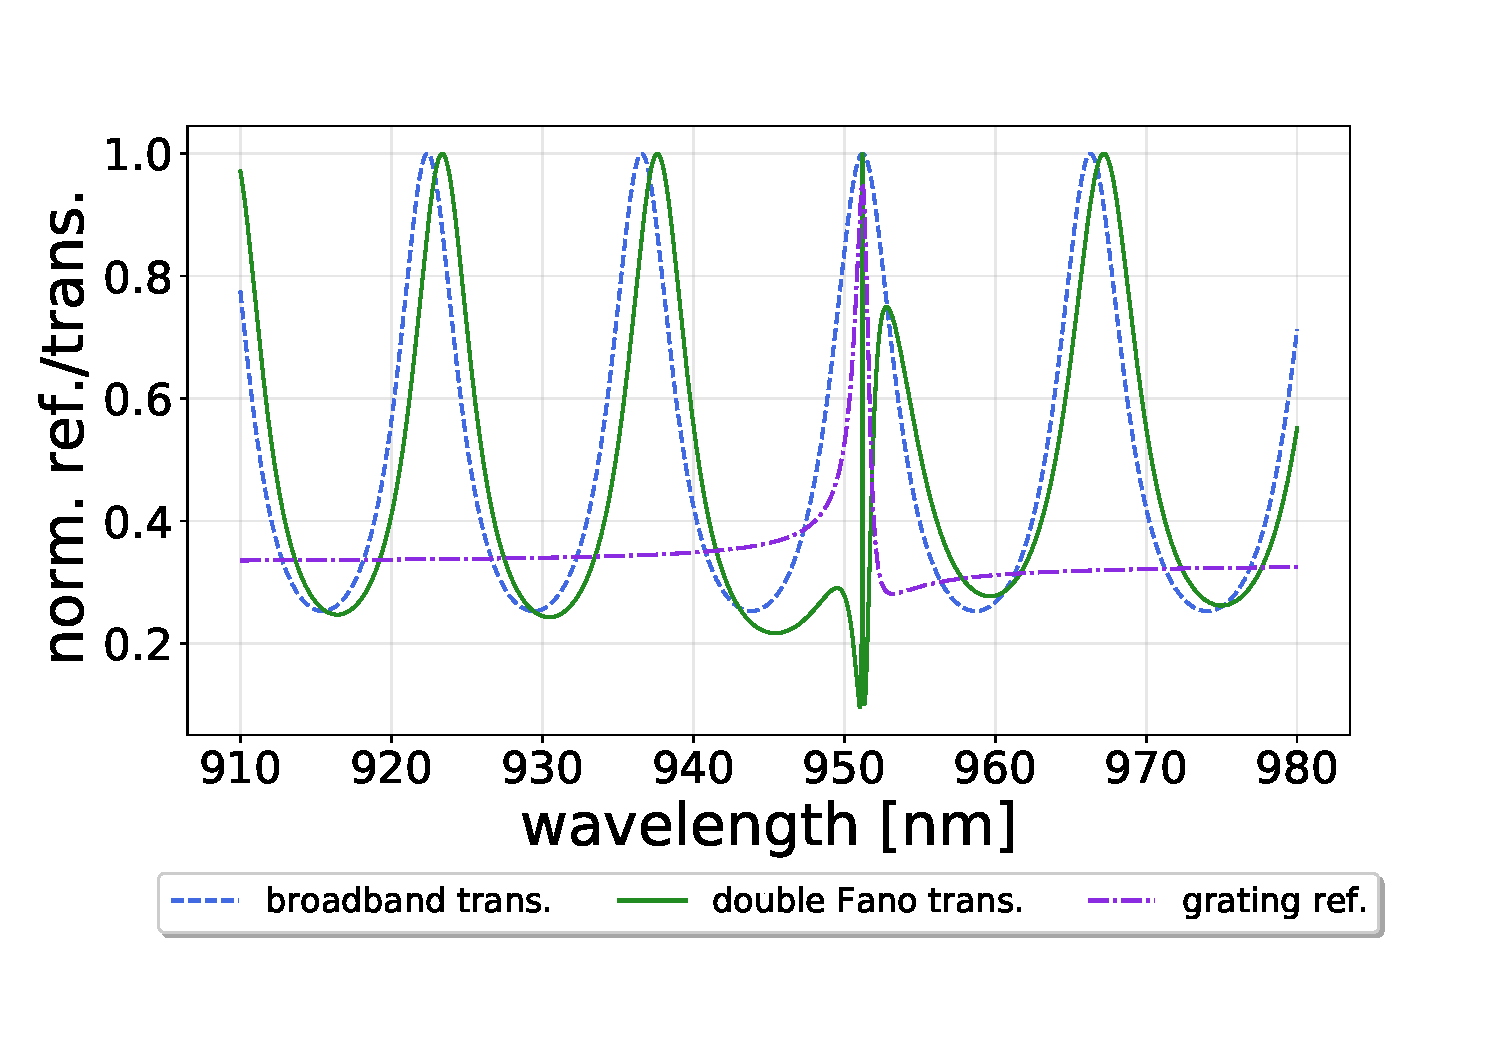
\includegraphics[width=\textwidth]{figures/double_fano_full_range_30um.pdf}
        \caption{}
        \label{fig:double_full_range}
    \end{subfigure}
    \begin{subfigure}[c]{0.49\textwidth}
        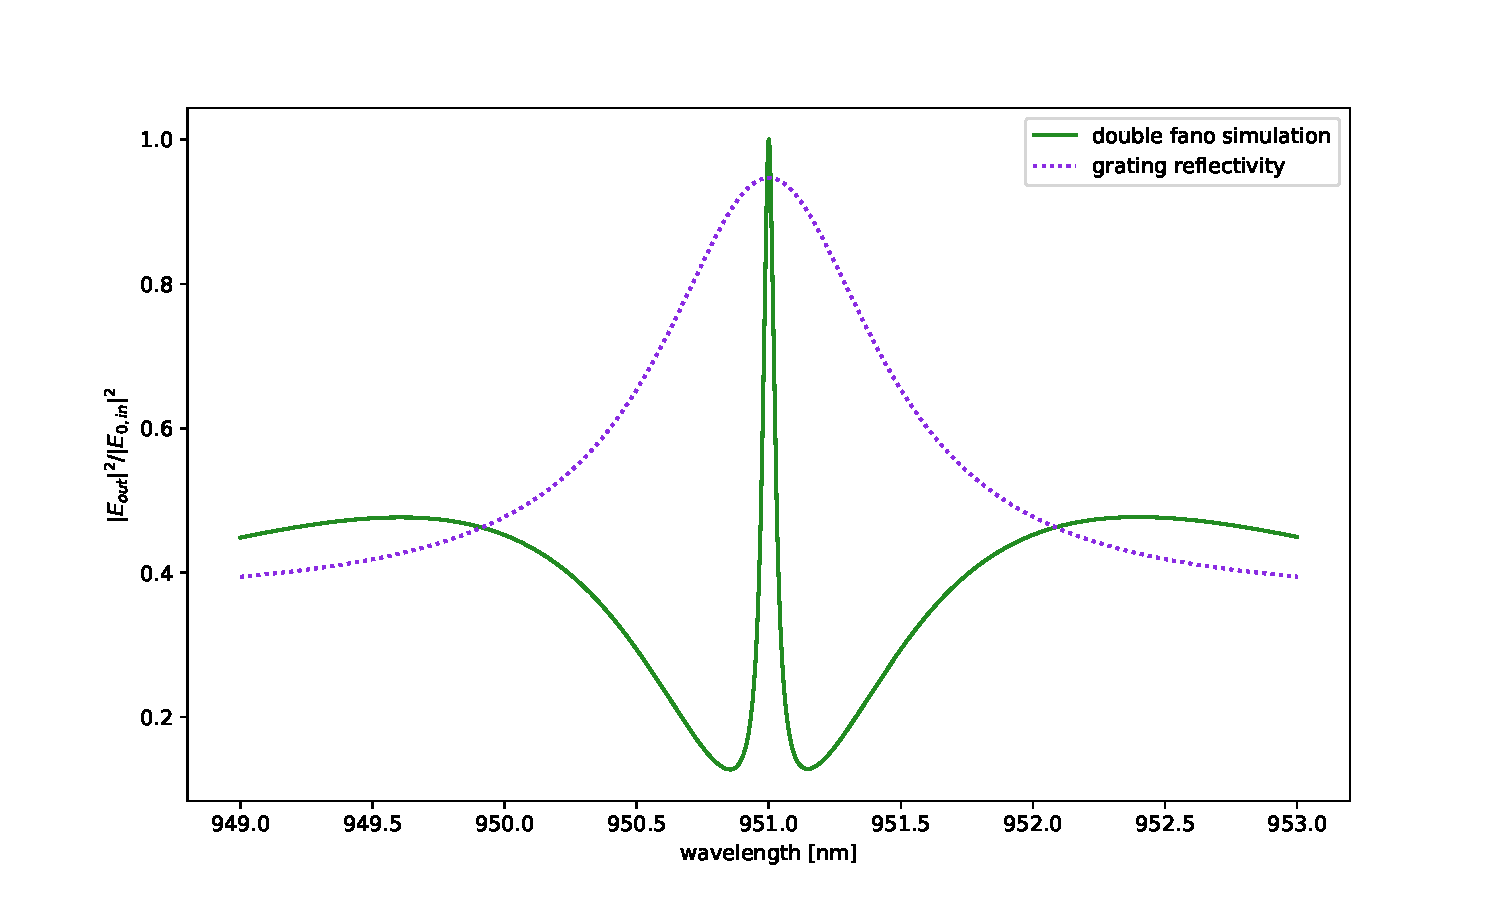
\includegraphics[width=\textwidth]{figures/double_fano_short_range_30um.pdf}
        \caption{}
        \label{fig:double_short_range}
    \end{subfigure}
    \caption{}
    \label{fig:double_fano_transmission}
\end{figure}

\subsubsection{Transmission linewidth}

\begin{equation}
    \delta \lambda \approx \frac{1}{\frac{1}{\delta \lambda_c} + \frac{1}{\delta \lambda_g^{double}}},
    \label{eq:analytical_linewidth_double}
\end{equation}

\begin{equation}
    \delta \lambda_c = \frac{\lambda_0^2}{8 \pi l} (|t_g(\lambda_0)|^2 + |t_m|^2 + L),
\end{equation}

\begin{equation}
    \delta \lambda_g^{double} = \frac{\gamma \lambda}{4 (1-r_d)}(|t_g(\lambda_0)|^2 + |t_m|^2 + L).
    \label{eq:double_fano_linewidth_contribution}
\end{equation}

\subsubsection{Single and double Fano cavity comparison}

Using the analytical expression for the double Fano cavity transmission in eq. (\ref{eq:analytical_linewidth_double}) we are now in a position to compare the single and double Fano cavities. Note that we at this point only consider the ideal case of the double Fano cavity where additional cavity losses are neglected and the two Fano mirrors used are identical, i.e. the cavity is said to be \emph{symmetrical}. The additional cavity losses are explicitly set to be given as
\begin{equation}
    L = 1-|r_g|^2-|t_g|^2 = 0.
\end{equation}

\begin{figure}[h!]
    \centering
    \begin{subfigure}[c]{0.49\textwidth}
        \centering
        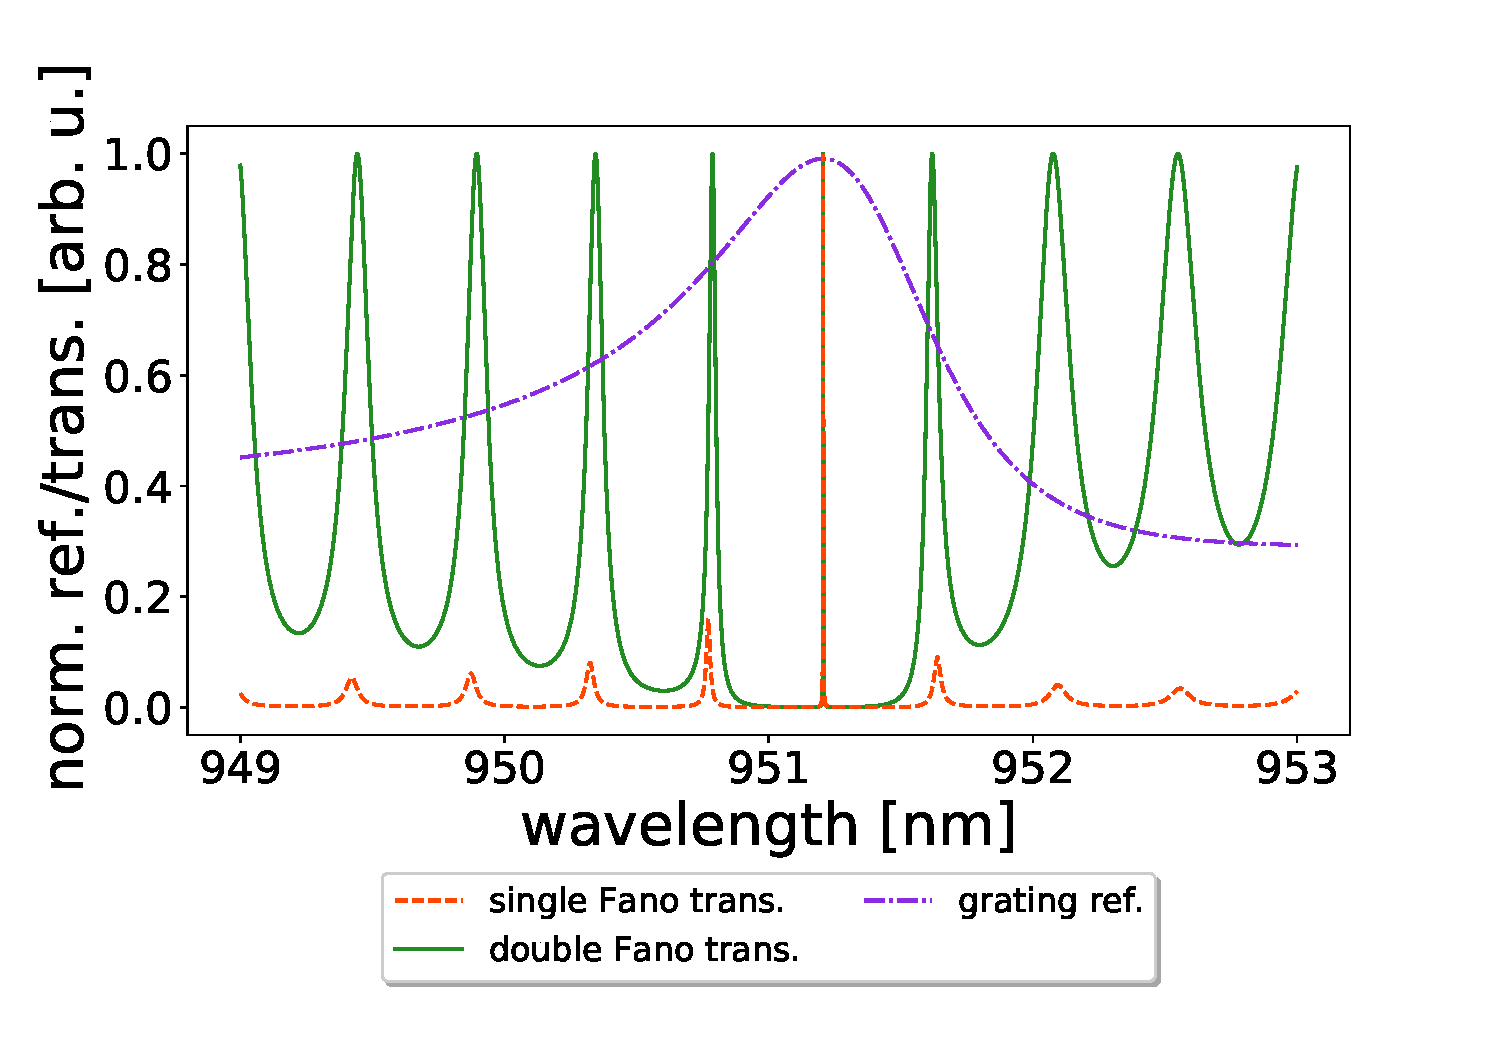
\includegraphics[width=\textwidth]{figures/single_and_double_1000um.pdf}
        \caption{}
        \label{fig:double_in_standard_regime}
    \end{subfigure}
    \begin{subfigure}[c]{0.49\textwidth}
        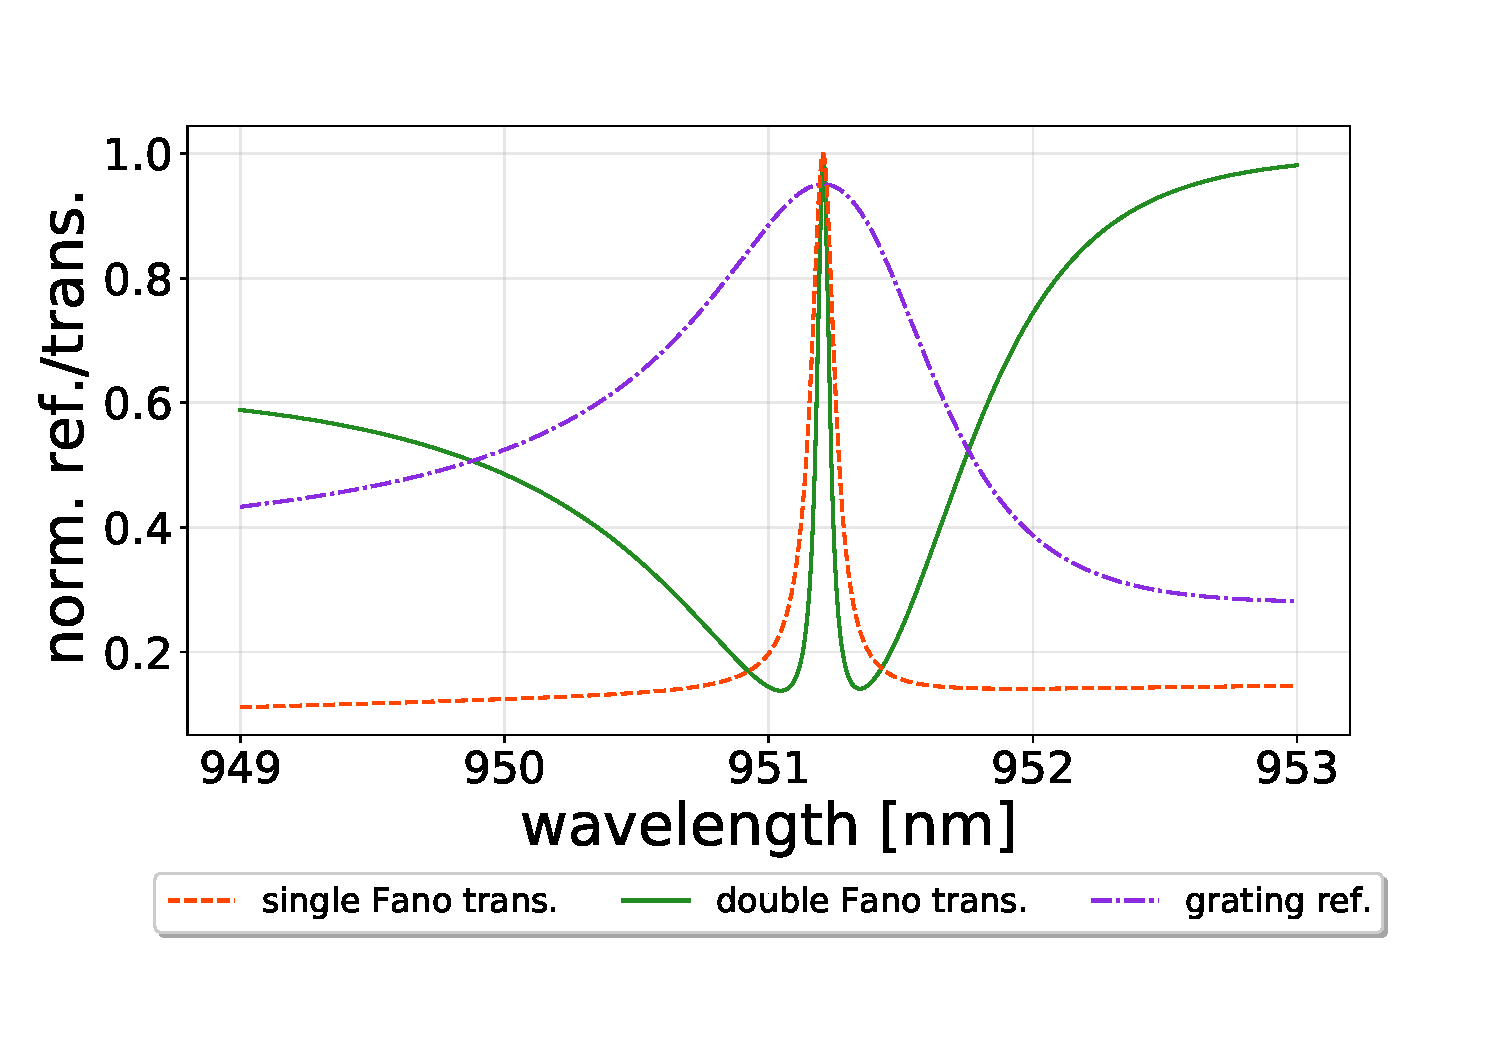
\includegraphics[width=\textwidth]{figures/single_and_double_5um.pdf}
        \caption{}
        \label{fig:double_in_fano_regime}
    \end{subfigure}
    \caption{}
    \label{fig:double_in_standard_and_fano_regimes}
\end{figure}

Figure \ref{fig:double_in_standard_and_fano_regimes} shows the transmission of the ideal double Fano cavity and the corresponding single Fano cavity for comparison. 

Figure \ref{fig:double_in_standard_regime} shows the transmission for a cavity length of $\sim 1000 \mu m$ which is well-inside the standard regime outlined in section \ref{sec:single_fano_cavity_trans_linewidth} where the standard broadband and single Fano cavities produce transmission spectra of almost identical linewidths. In this regime, due to the $1/l$ proportionality of the FSR, the off-resonance behavior of the double Fano cavity transmission is visible in the range plottet. It is seen, contrary to the single Fano cavity, that the transmission at each cavity resonance reaches a normalized transmission of $|E_{out}|^2/|E_{0,in}|^2=1$. This is due to the fact that the two gratings, while they have wavelength dependent transmission and reflectivity coefficients, always have identical ones for the ideal case which maximizes the Fabry-Perot transmission function and ensures unity transmission at any cavity resonance. The minimum level of the cavity changes according to the reflectivity of the Fano mirrors and by that the HWHM also changes as we move further from the guided-mode resonance. Both the minimum transmission level and the HWHM converge when moving away from the resonance wavelength, when the reflectivity becomes constant. 

Figure \ref{fig:double_in_fano_regime} shows the transmission of a double Fano cavity of length $\sim 5 \mu m$ which, contrary to the one in figure \ref{fig:double_in_standard_regime}, is well within the Fano regime. It is seen that the double Fano cavity transmission produces a resonance peak with a HWHM narrower than the one for the single Fano cavity, as is predicted in eq. (\ref{eq:double_fano_linewidth_contribution}). Furthermore, the immediate off-resonance behavior of the double Fano cavity transmission in the Fano regime, is drastically different than for the single Fano cavity. This is due to the collective higher transmission in this region compared with the single Fano case where the broadband mirror has a constant, and often high, reflectivity and hence a correspondingly low transmission.

\begin{figure}[h!]
    \centering
    \begin{subfigure}[c]{0.64\textwidth}
        \centering
        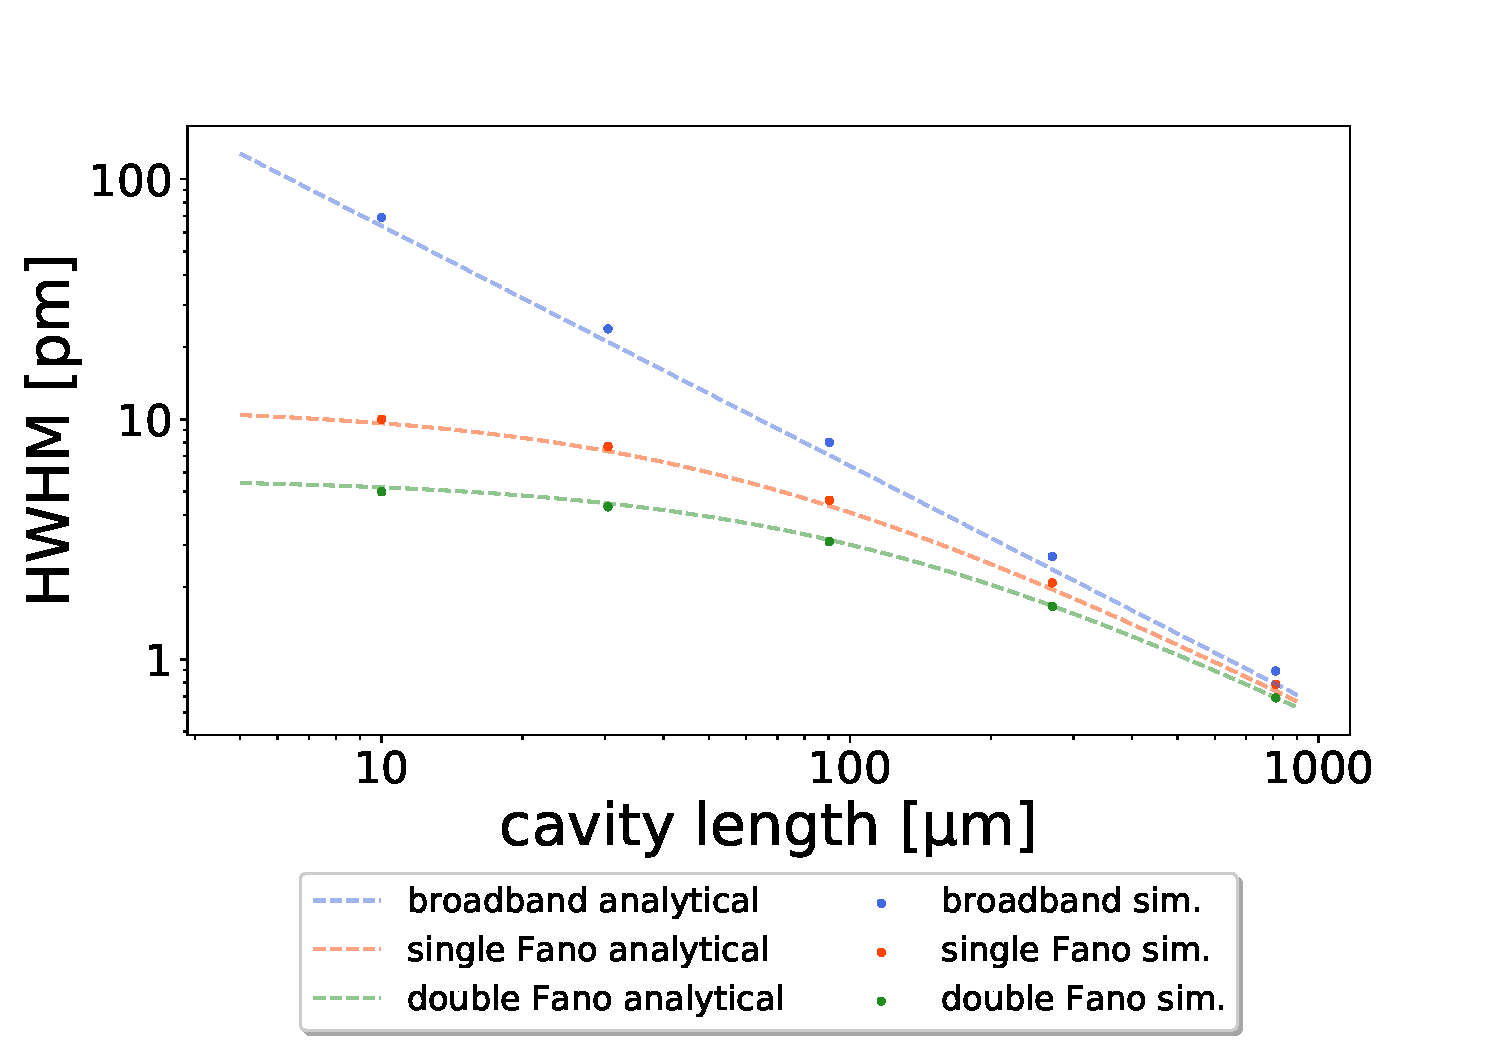
\includegraphics[width=\textwidth]{figures/HWHM_broadband_vs_single_vs_double_sim.pdf}
        \caption{The analytical resonance linewidths (eqs. (\ref{eq:analytical_linewidth}), (\ref{eq:analytical_linewidth_double}), and (\ref{eq:analytical_linewidth_broadband})) as a function of the cavity length for the broadband, single and double Fano cavities are shown together with linewidths of corresponding transmission profiles simulated using eqs. (\ref{eq:single_fano_trans}), (\ref{eq:double_fano_transmission}), and (\ref{eq:fabry_perot_trans}) for comparison.}
        \label{fig:HWHM_double_vs_single_vs_broadband}
    \end{subfigure}
    \begin{subfigure}[c]{0.34\textwidth}
        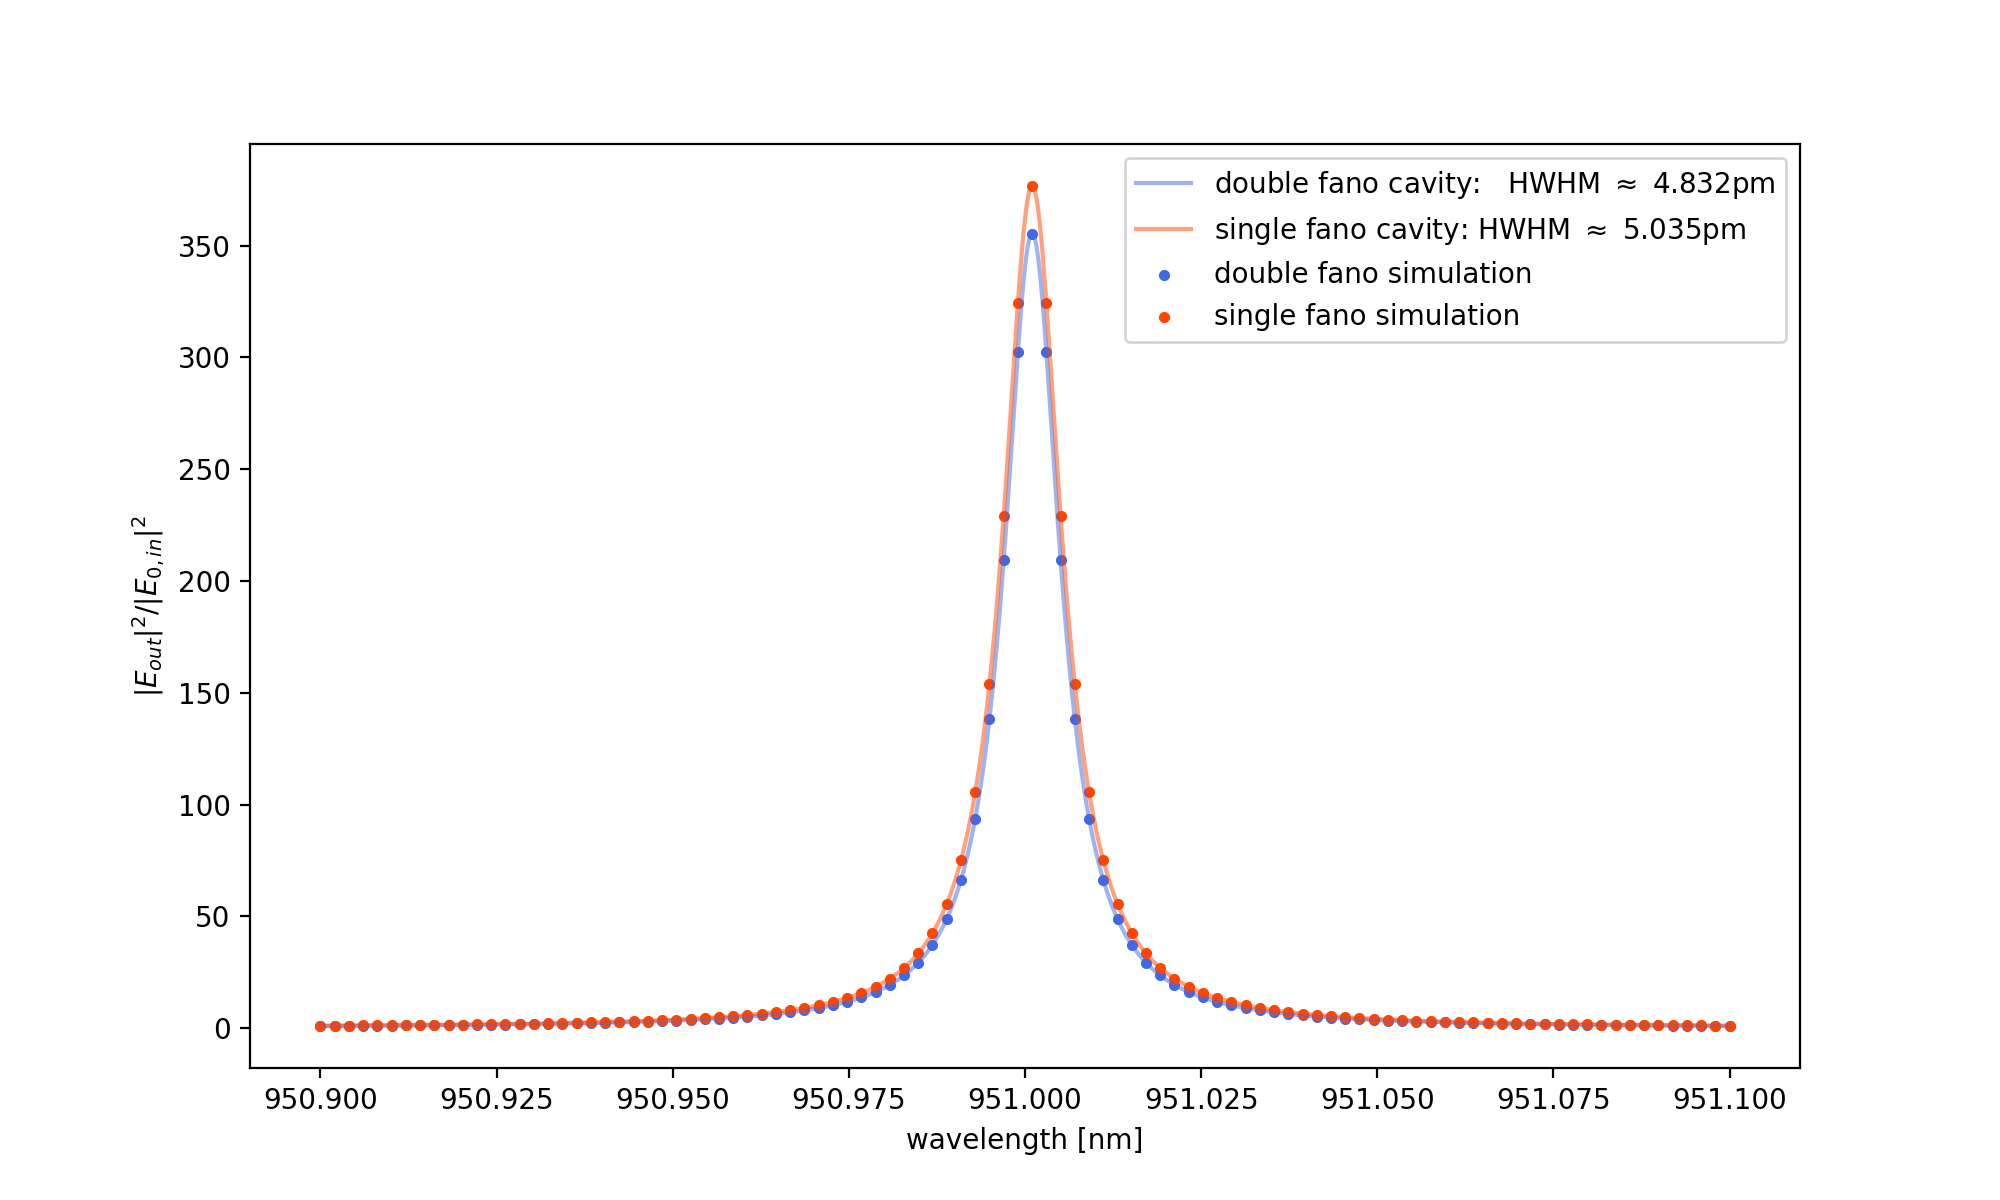
\includegraphics[width=\textwidth]{figures/sim_single_vs_double_700um.png}
        \caption{Intracavity transmission spectra of single and double Fano cavities of length $\sim 700 \mu m$.}
        \label{fig:700um_double_and_single_fano_peak}
        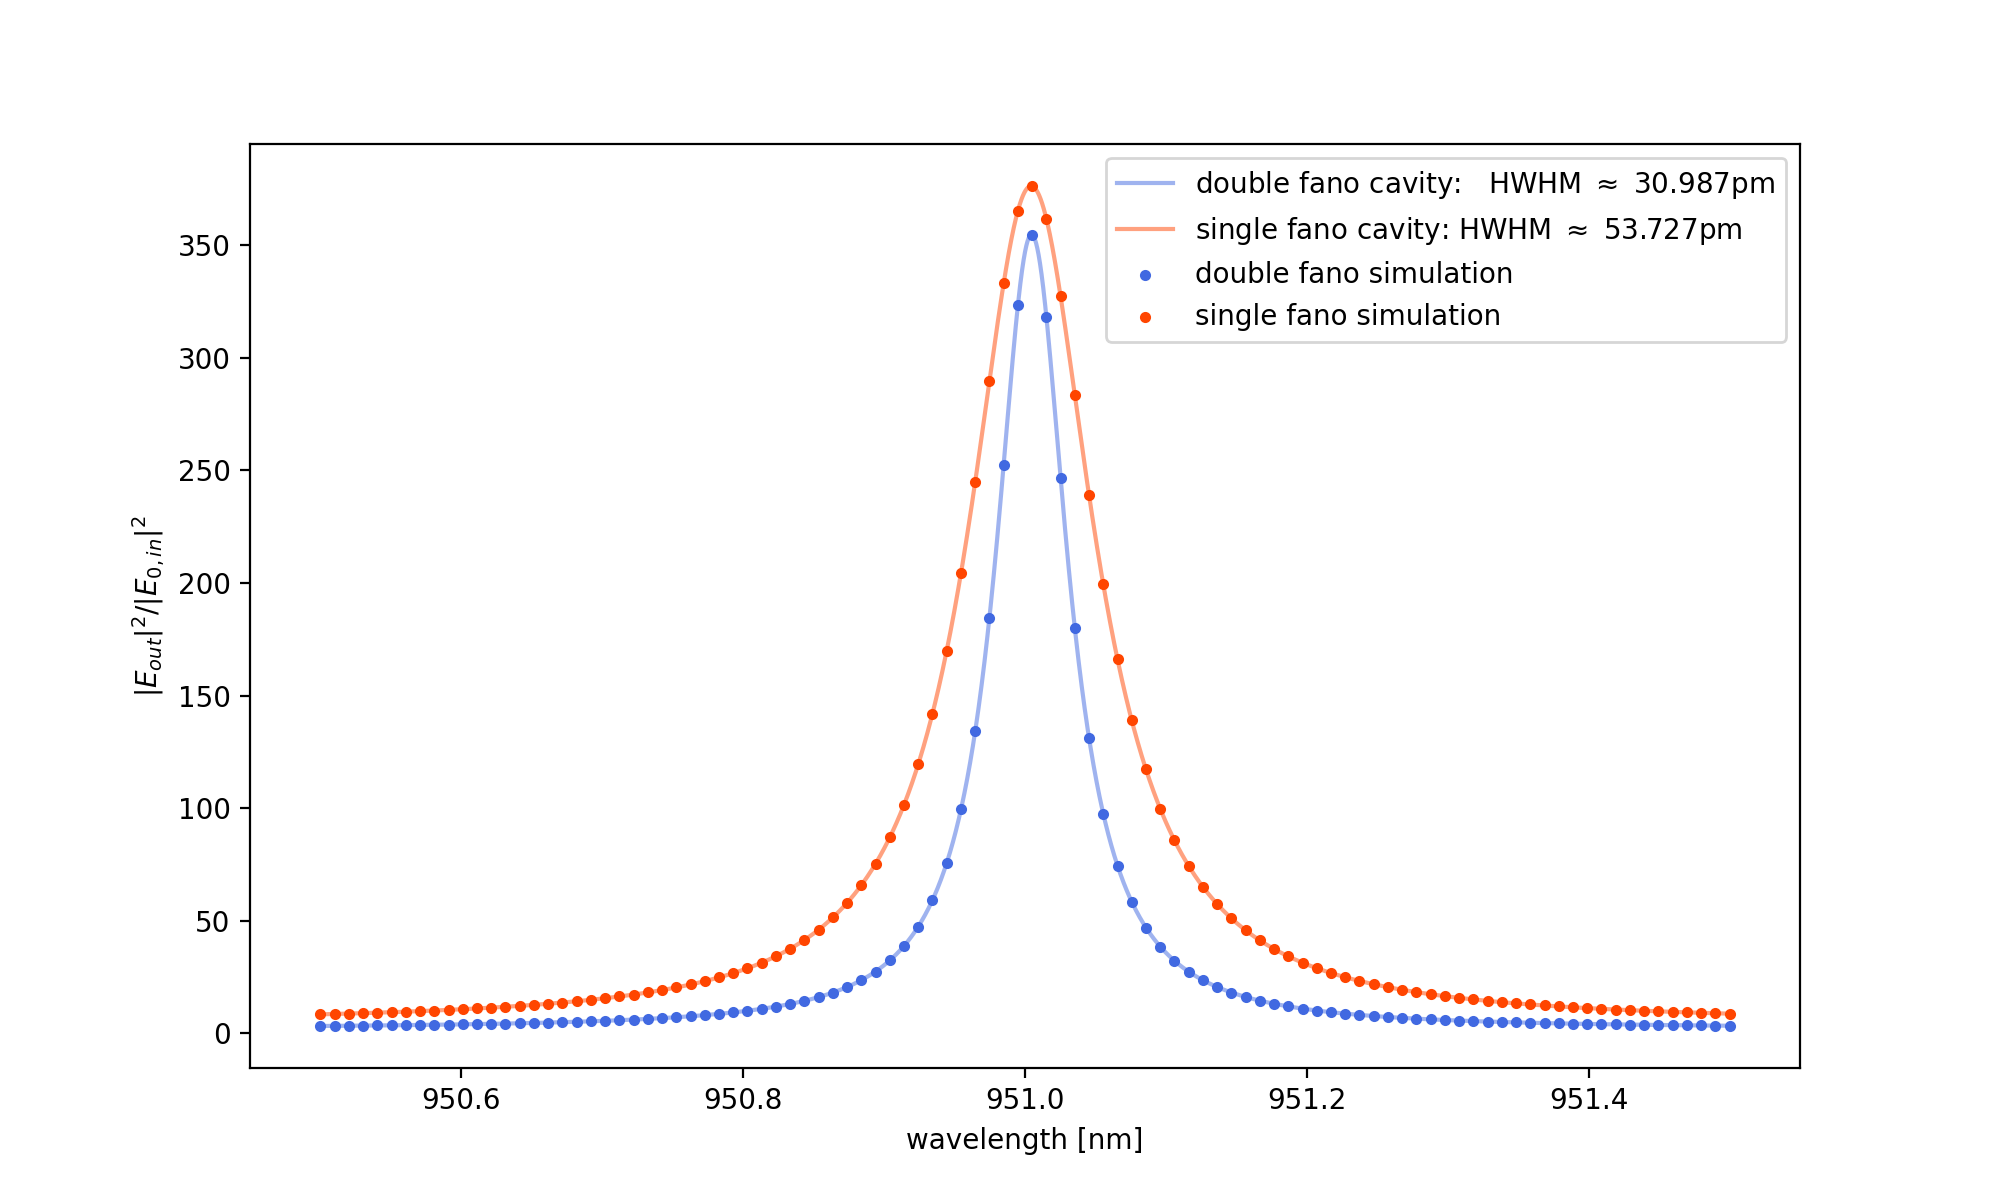
\includegraphics[width=\textwidth]{figures/sim_single_vs_double_10um.png}
        \caption{Intracavity transmission spectra of single and double Fano cavities of length $\sim 10 \mu m$.}
        \label{fig:10um_double_and_single_fano_peak}
    \end{subfigure}
\end{figure}

Figure \ref{fig:HWHM_double_vs_single_vs_broadband} shows the analytical linewidth calculated and compared for the broadband, single Fano, and double Fano cavities, calculated using eqs. (\ref{eq:analytical_linewidth_broadband}), (\ref{eq:analytical_linewidth}), (\ref{eq:analytical_linewidth_double}). These are compared with linewidths found as fitting parameters from a least squares fit of the general Fano transmission formula given in eq. (\ref{eq:general_fano_model}) to transmission spectra calculated using eqs. (\ref{eq:fabry_perot_trans}), (\ref{eq:single_fano_trans}), and (\ref{eq:double_fano_transmission}). According to eq. (\ref{eq:analytical_linewidth_double}) the linewidth of the double Fano cavity transmission should converge to exactly half that of the single Fano cavity, meaning that
\begin{equation}
    \delta \lambda_{double} = \frac{\delta \lambda_{single}}{2}, \hspace{0.5cm} \text{for } l \rightarrow 0.
\end{equation}
This is supported well by the simulation depicted in figure \ref{fig:HWHM_double_vs_single_vs_broadband}.

Figures \ref{fig:700um_double_and_single_fano_peak} and \ref{fig:10um_double_and_single_fano_peak} contain examples of intracavity\footnote{The reason these are shown as intracavity spectra instead of transmission spectra is due to the immediate off-resonance behavior of the double Fano cavity transmission. The shape makes accurate fitting a challenge, and while the intracavity spectra cannot be measured in the lab, the linewidth when simulated is identical to the resulting transmission peaks.} spectra of single and double Fano cavities and corresponding fits to the general Fano model in order to determine their linewidths. 

\subsubsection{Additional cavity losses}

Thus far we have only examined a lossless double Fano cavity where
\begin{equation}
    |r_g|^2 + |t_g|^2 = 1
\end{equation}
is fulfilled for both Fano mirrors used to contruct the cavity.

In this section we will investigate what happens when we introduce additional cavity losses\footnote{Not to be confused with the often used definition of cavity losses given as $L=1-|r|^2$ where anything not being reflected back into the cavity is considered to have a contribution to the losses.}
\begin{equation}
    L = 1 - |r_g|^2 - |t_g|^2,
\end{equation}
leading to the modified condition
\begin{equation}
    |r_g|^2 + |t_g|^2 + L = 1.
\end{equation}

\begin{figure}[h!]
    \centering
    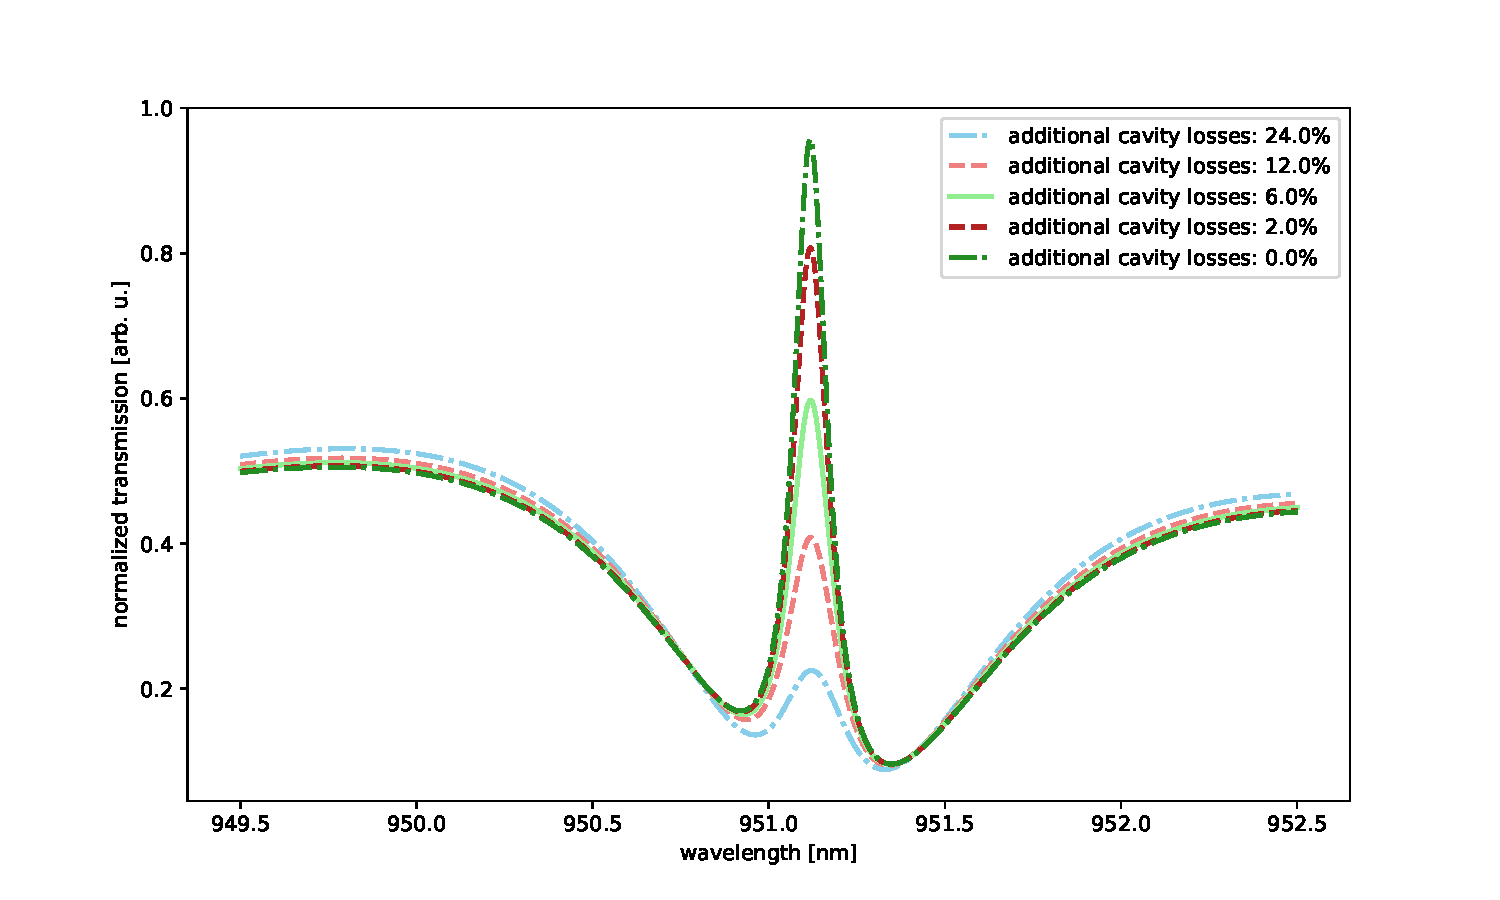
\includegraphics[width=0.6\textwidth]{figures/double_fano_loss_scan.pdf}
    \caption{}
    \label{fig:double_loss_scan}
\end{figure}

Figure \ref{fig:double_loss_scan} shows double Fano transmisison spectra as a function of wavelength for a symmetric cavity with varying values for the additional cavity losses. It is readily seen that the maximum value reached in each spectrum is rapidly reduced with the introduction of these losses. 

Since the linewidth is defined as the HWHM of the transmission profile, this will naturally vary as a function of additional cavity losses. This is depicted in figure \ref{fig:HWHM_vs_losses} where the HWHM is shown for different values of $L$. Examples of intracavity spectra taken for different values of $L$ are shown in figures \ref{fig:HWHM_vs_losses_whole_figure}b and \ref{fig:HWHM_vs_losses_whole_figure}c, along with their respective least squares fits to the general Fano model in eq. (\ref{eq:general_fano_model}) and linewidths found as fitting parameters hereof. 

\begin{figure}[h!]
    \centering
    \begin{subfigure}[c]{0.64\textwidth}
        \centering
        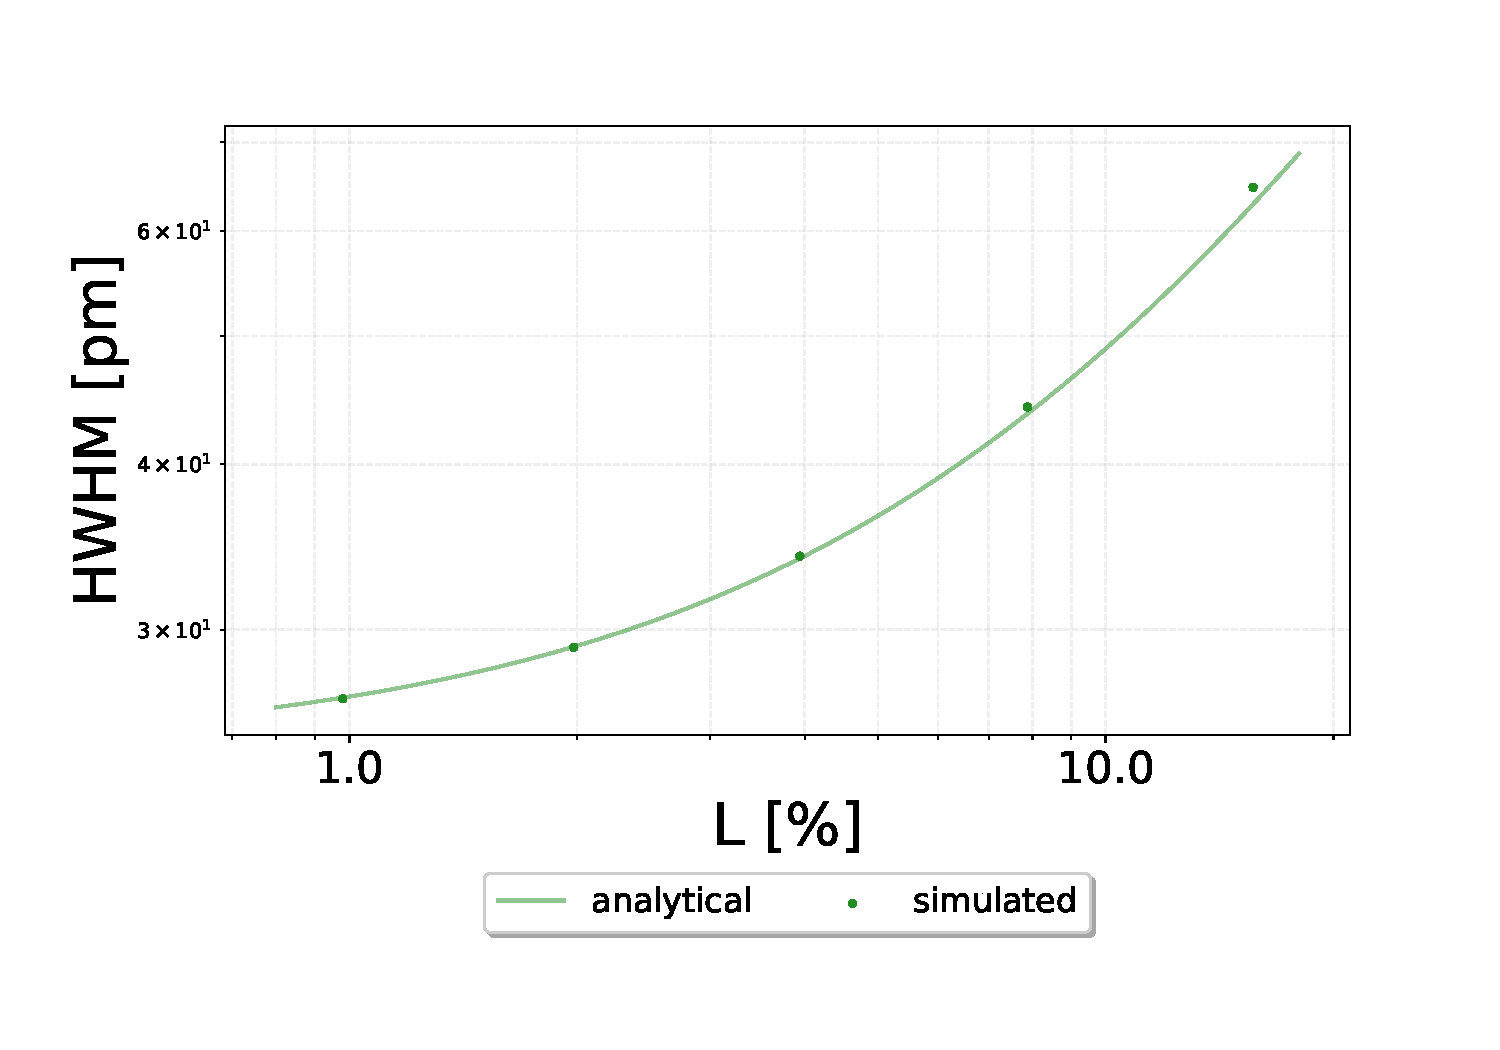
\includegraphics[width=\textwidth]{figures/linewidth_vs_losses.pdf}
        \caption{HWHM of a symmetric $\sim 30 \mu m$ double Fano cavity as a function of additional cavity losses $L = 2(|r_g|^2 - |t_g|^2)$. Improve this figure by adding the analytical prediction of the linewidth as a function of losses.}
        \label{fig:HWHM_vs_losses}
    \end{subfigure}
    \begin{subfigure}[c]{0.34\textwidth}
        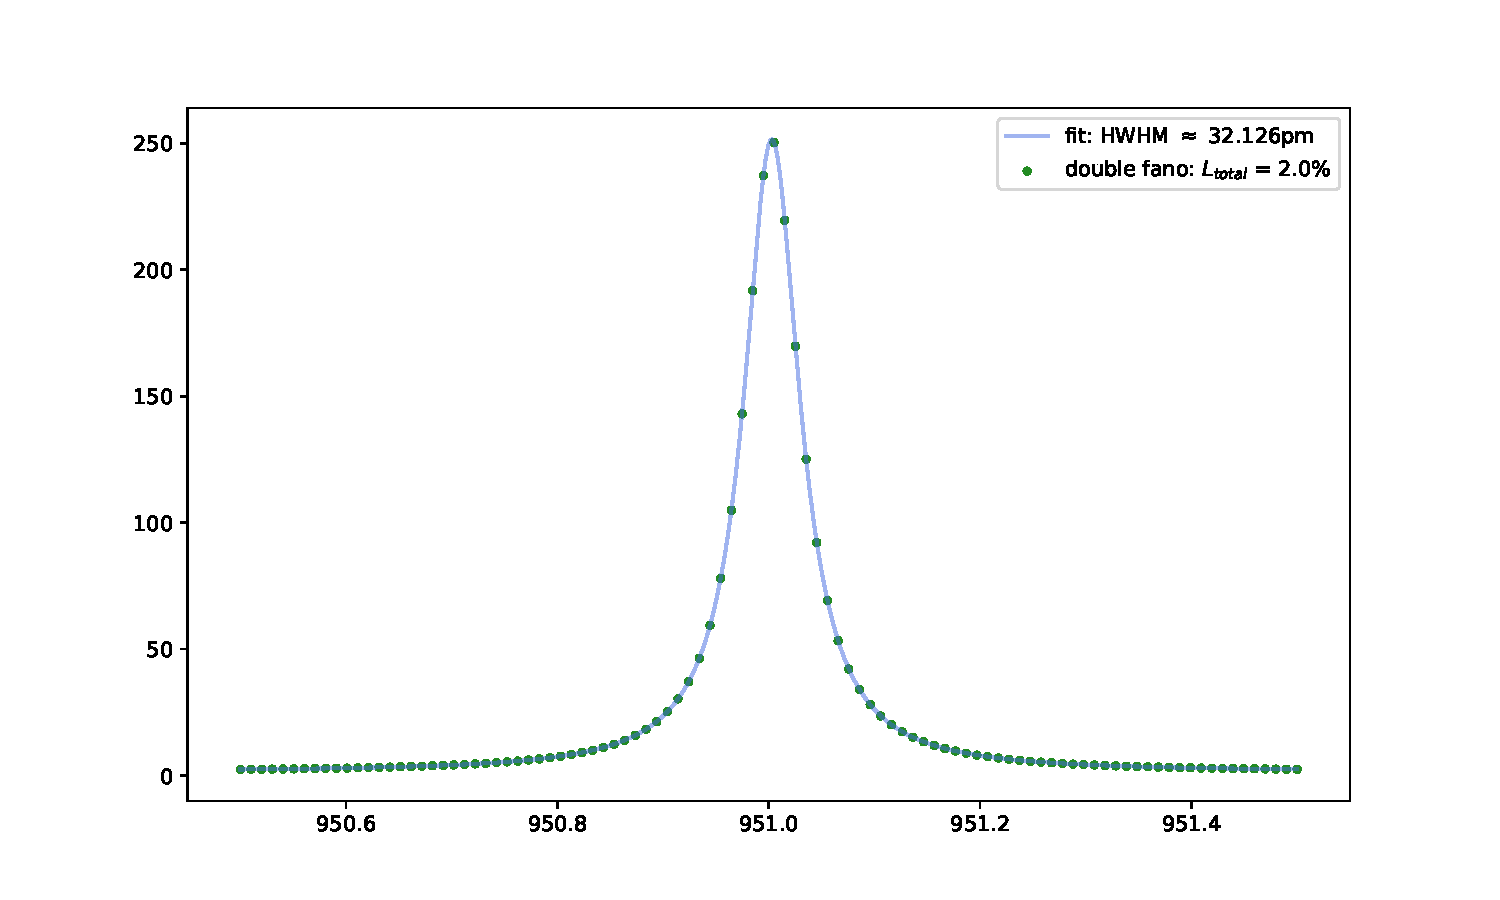
\includegraphics[width=\textwidth]{figures/double_2_loss_30um.pdf}
        \caption{Double Fano transmission spectra with cavity length $\sim 30 \mu m$ and $L = 2\%$.}
        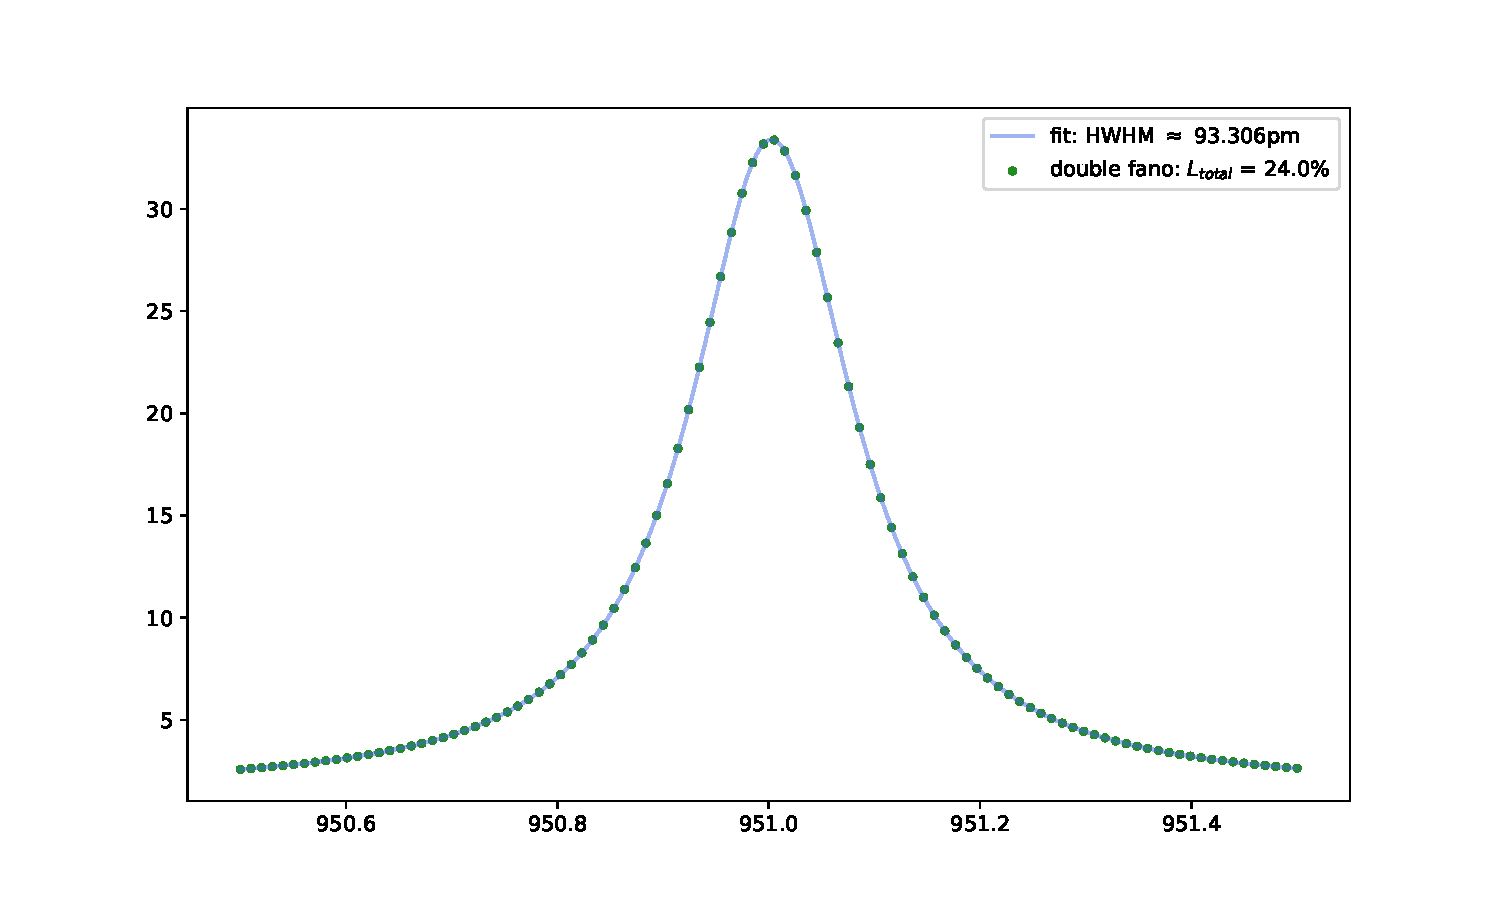
\includegraphics[width=\textwidth]{figures/double_24_loss_30um.pdf}
        \caption{Double Fano transmission spectra with cavity length $\sim 30 \mu m$ and $L = 24\%$.}
    \end{subfigure}
    \caption{}
    \label{fig:HWHM_vs_losses_whole_figure}
\end{figure}

Figure \ref{fig:HWHM_vs_losses} shows the simulated linewidths of intracavity spectra as a function of total cavity losses $L$, and is compared with the analytical formula for the double Fano linewidth in eq. (\ref{eq:analytical_linewidth_double}). It is seen that the analytical model proves, once again, to be a powerful predicting technique for the linewidth, and especially for cavities with relatively low losses. 

\subsubsection{Spectral and spacial detuning - $l_{g} \geq l \geq l_{g}^{\prime}$ \& $\Delta \neq 0$ (lossless double fano cavity)}

Up until this point, it has been assumed that the Fano mirrors making up the double Fano cavity has been identical, namely the cavity has been \emph{symmetric}. However, in practice this is very unlikely to be the case, as any Fano mirror constructed is bound to have some uncertainties attached to the physical parameters describing it. For that reason we investigate the effect of an \emph{assymetric} cavity on the resulting transmission profile. Here we remember that each sub-wavelength grating is describes by a set of parameters, $\lambda_0$, $\lambda_1$, $t_d$, $\gamma \lambda$ and $\beta$, which respectively describe the cavity resonance wavelength, guided-mode resonance wavelength, direct transmission, guided-mode resonance linewidth and additional losses of each grating. In order to model only a spectral detuning, we therefore simply change the parameters regarding the cavity and guided-mode resonance wavelengths, $\lambda_0$ and $\lambda_1$ by an amount corresponding to the detuning we wish to study. For this section the parameters will be given as
\begin{equation}
    \begin{split}
    \lambda_0 = &951 nm,\:\: \lambda_1 = 951 nm,\:\: t_d = 80\%,\\ &\gamma \lambda = 0.5 nm\: \text{ and }\: \beta = 10^{-6}
    \end{split}
    \label{eq:grating_params}
\end{equation}
for the unchanged Fano mirror, and
\begin{equation}
    \begin{split}
    \lambda_0^{\prime} = &\lambda_0 + \Delta,\:\: \lambda_1^{\prime} = \lambda_1 + \Delta,\:\: t_d^{\prime} = t_d,\\ &\gamma \lambda^{\prime} = \gamma \lambda\: \text{ and }\: \beta^{\prime} = \beta
    \end{split}
    \label{eq:detuned_grating_params}
\end{equation}
for the \emph{detuned} Fano mirror. Figure \ref{fig:detuned_grating_spectra} shows the normalized reflectivity and transmission spectra of the Fano mirrors described by the parameters described in eqs. (\ref{eq:grating_params}) and (\ref{eq:detuned_grating_params}).

\begin{figure}[h!]
    \centering
    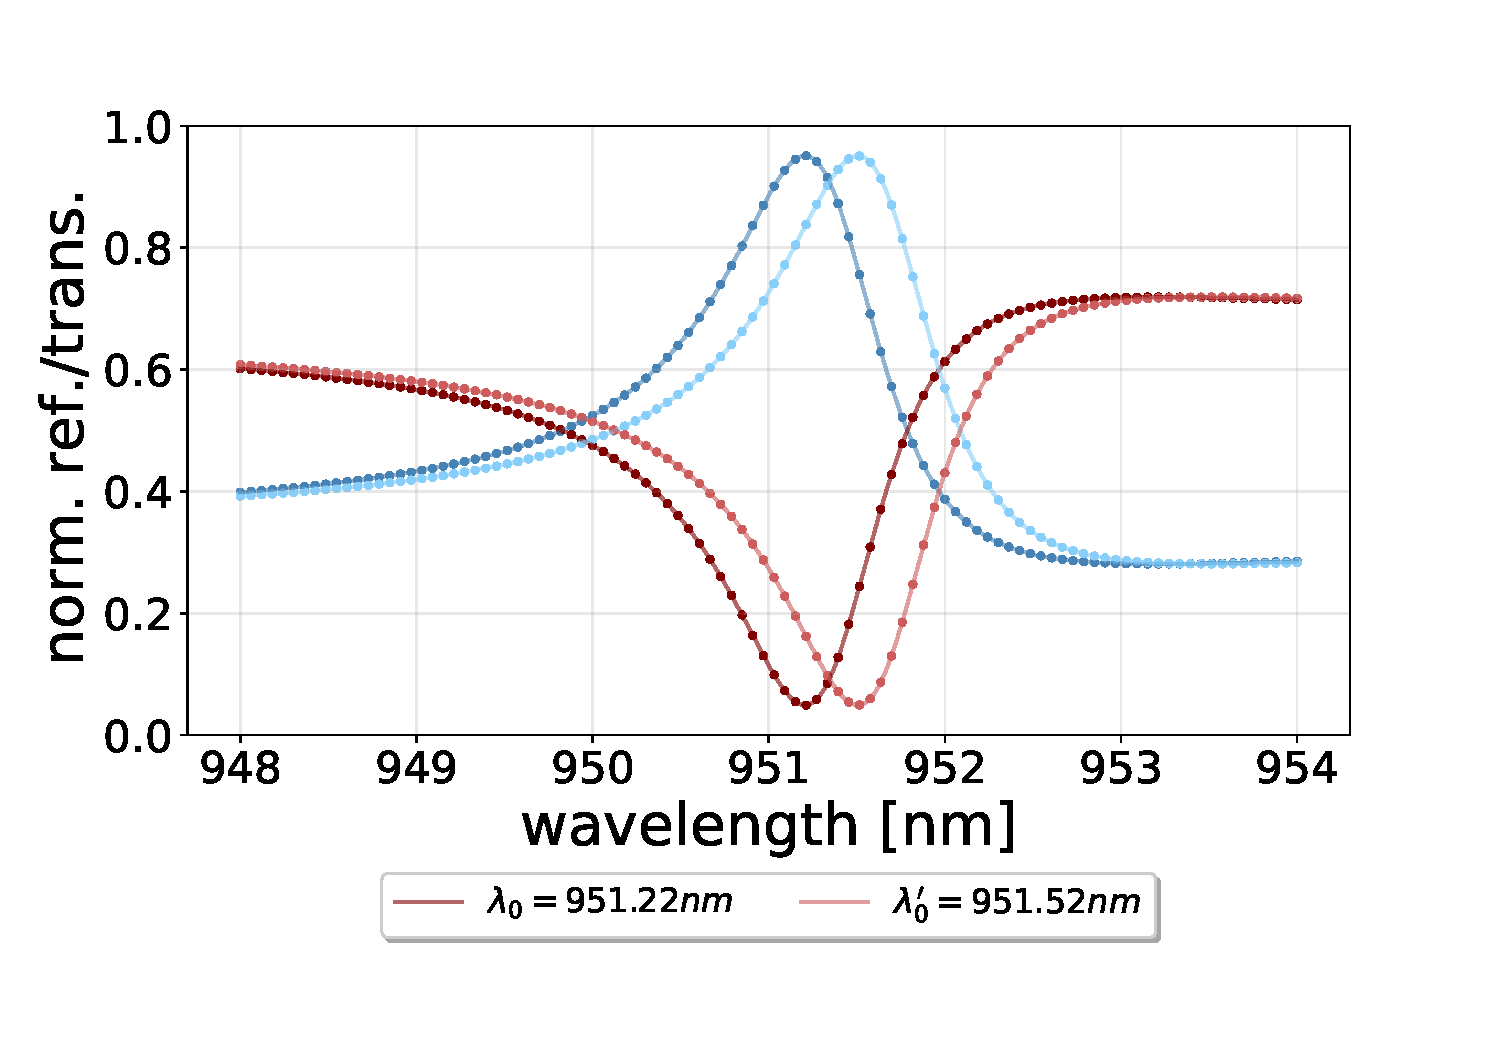
\includegraphics[width=0.7\textwidth]{figures/detuned_grating_spectra.pdf}
    \caption{The normalized reflectivity and transmission spectra of the Fano mirrors described in eqs. (\ref{eq:grating_params}) and (\ref{eq:detuned_grating_params}) for a detuning given as $\Delta = 0.3nm$.}
    \label{fig:detuned_grating_spectra}
\end{figure}

As has been observed in previous sections, the Fano resonance transmission peak is present at the point where the grating reflectivity $r_g(\lambda)$ is maximized and transmission $t_g(\lambda)$ minimized. However, when $\lambda_0 \neq \lambda_0^{\prime}$ and $\lambda_1 \neq \lambda_1^{\prime}$, this is no longer a trivial conclusion to draw. The question of whether the cavity resonance should be tuned to match the guided-mode resonance wavelength of one grating or the other, or maybe somewhere in between does not have an obvious answer. This will be further expanded upon later in this section, but in order to move forward with the investigation of the spectral detuning we, for now, accept that the optimal cavity length, is the one corresponding to a cavity resonance $\lambda_t$ given, exactly between the two guided-mode resonance wavelengths, as 
\begin{equation}
    \lambda_t = \frac{\lambda_{0,1} + \lambda_{0,1}^{\prime}}{2}.
    \label{eq:transmission_wavelength}
\end{equation}
The subscribt \emph{0,1} indicate that the two are interchangable, as the two are assumed identical at this time, and \emph{t} is for \emph{transmission} as this is, later on, to be used experimentally as the \emph{transmission wavelength}. 

\begin{figure}[h!]
    \centering
    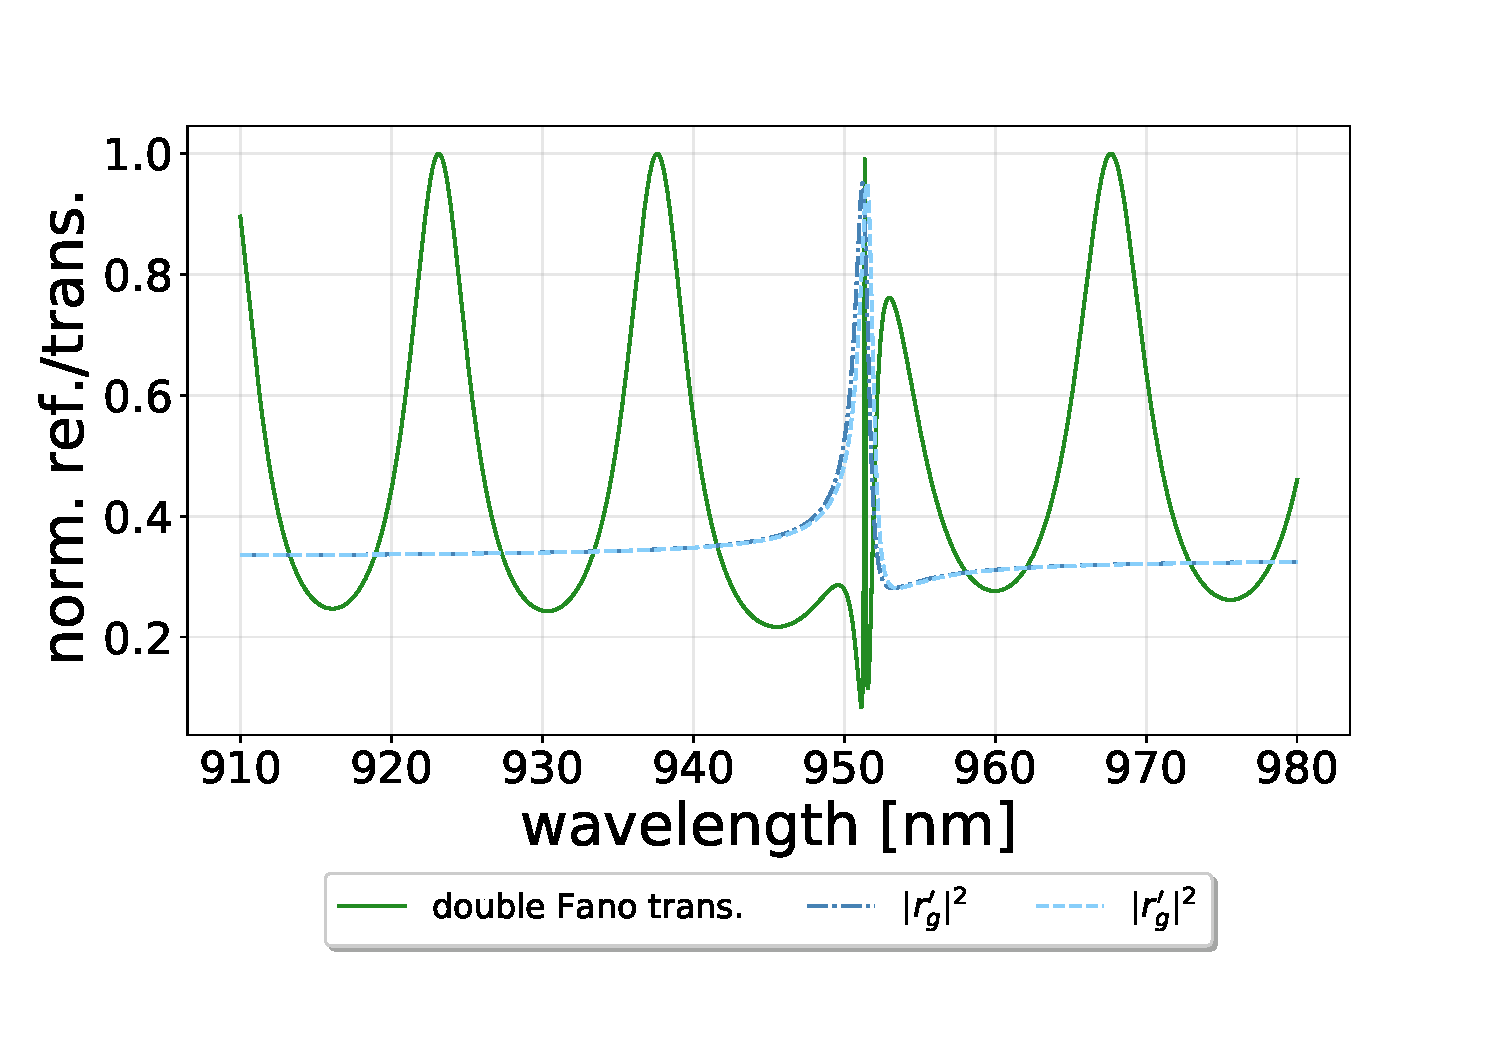
\includegraphics[width=0.7\textwidth]{figures/detuned_full_range_double_trans.pdf}
    \caption{The double Fano transmission spectra of a cavity detuned by $\Delta = 0.3nm$, as seen in figure \ref{fig:detuned_grating_spectra}, together with the reflectivity and transmission spectra of the Fano mirrors used for the simulation.}
    \label{fig:detuned_double_fano_transmission}
\end{figure}

Figure \ref{fig:detuned_double_fano_transmission} shows the transmission spectrum of a detuned double Fano cavity with parameters corresponding to the transmission and reflectivity spectra in figure \ref{fig:detuned_grating_spectra}, meaning that $\Delta = 0.3nm$. The transmission wavelength $\lambda_t$ is chosen such that eq. (\ref{eq:transmission_wavelength}) is fulfilled, and correspndingly it is seen that the transmission peak is placed exactly between the maximum (minimum) reflectivites (transmissions) of the two grating, i.e. between the two guided-mode resonance wavelengths. Furthermore, it can be concluded that the detuning is chosen such that the overlap between the guided-mode resonances is still substantiel enough for them to couple and hence for the the overall Fano resonance to be excited. 

While knowing that a detuning of $0.3nm$ is acceptable in terms of exciting the Fano resonance in the lossless case, it does not provide much in terms of estimating the acceptable detuning for any experimental purposes. In figure \ref{fig:detuning_scan} the double Fano transmission is shown for increasing detuning $\Delta$ and transmission wavelength $\lambda_t = (\lambda_{0,1} + \lambda_{0,1}^{\prime})/2$. 

\begin{figure}[h!]
    \centering
    \begin{subfigure}[b]{0.49\textwidth}
        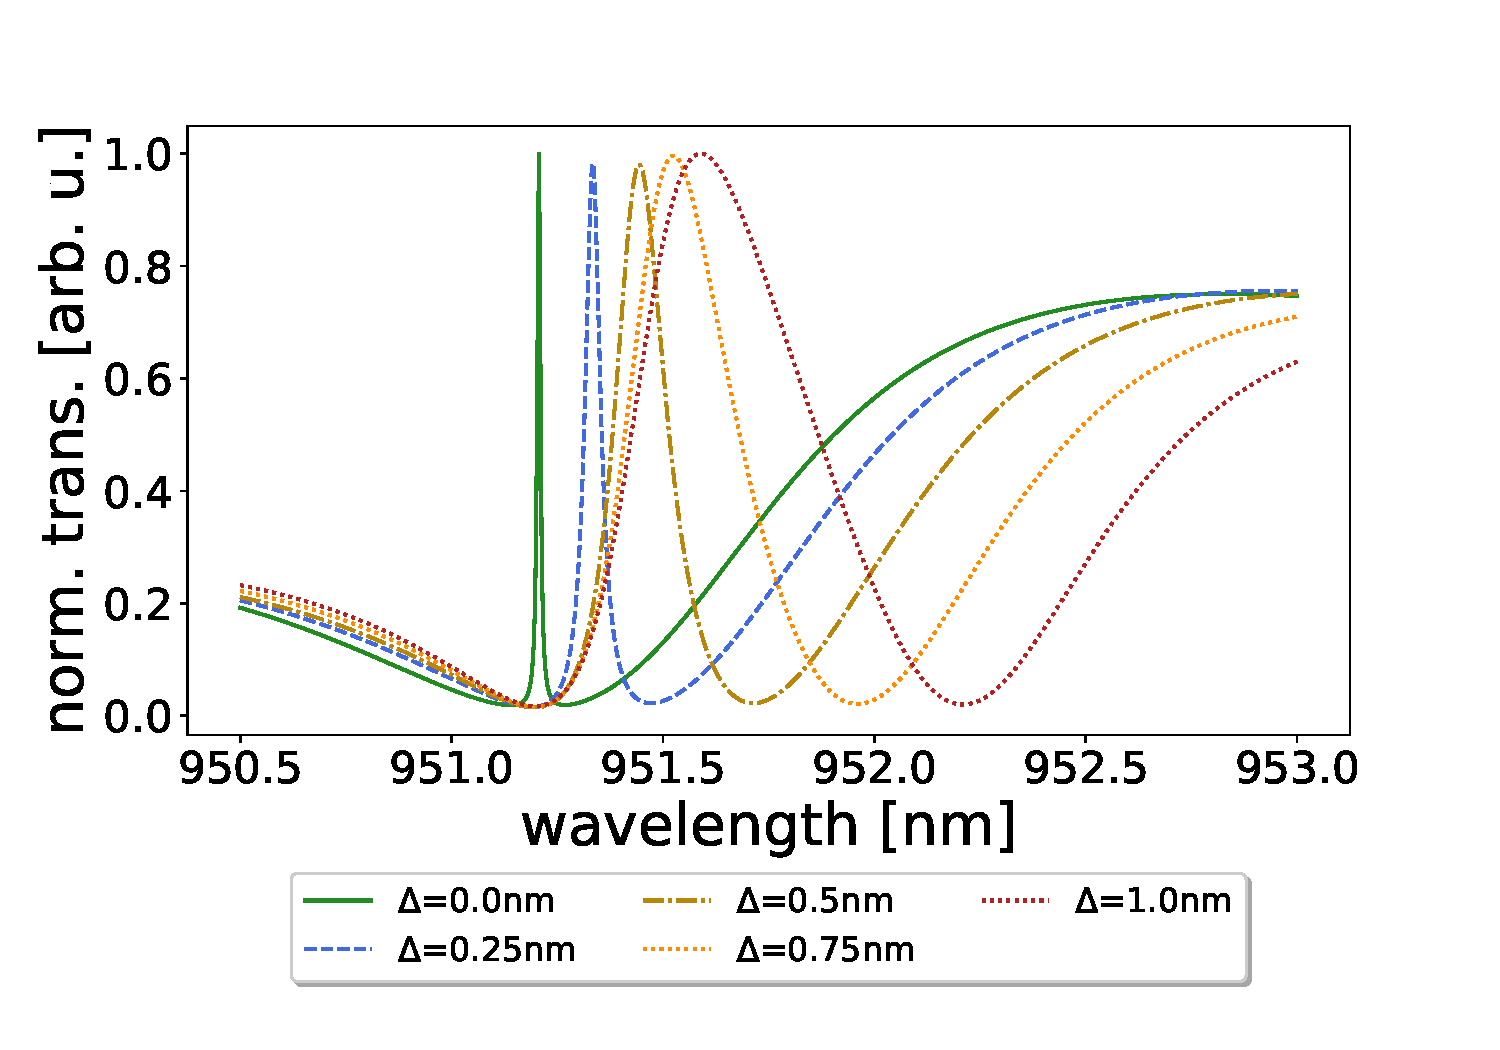
\includegraphics[width=\textwidth]{figures/detuning_scan_double_fano_30um.pdf}
        \caption{Double Fano cavity transmission spectra for different values of the spectral detuning $\Delta$.}
        \label{fig:detuning_scan}
    \end{subfigure}
    \begin{subfigure}[b]{0.49\textwidth}
        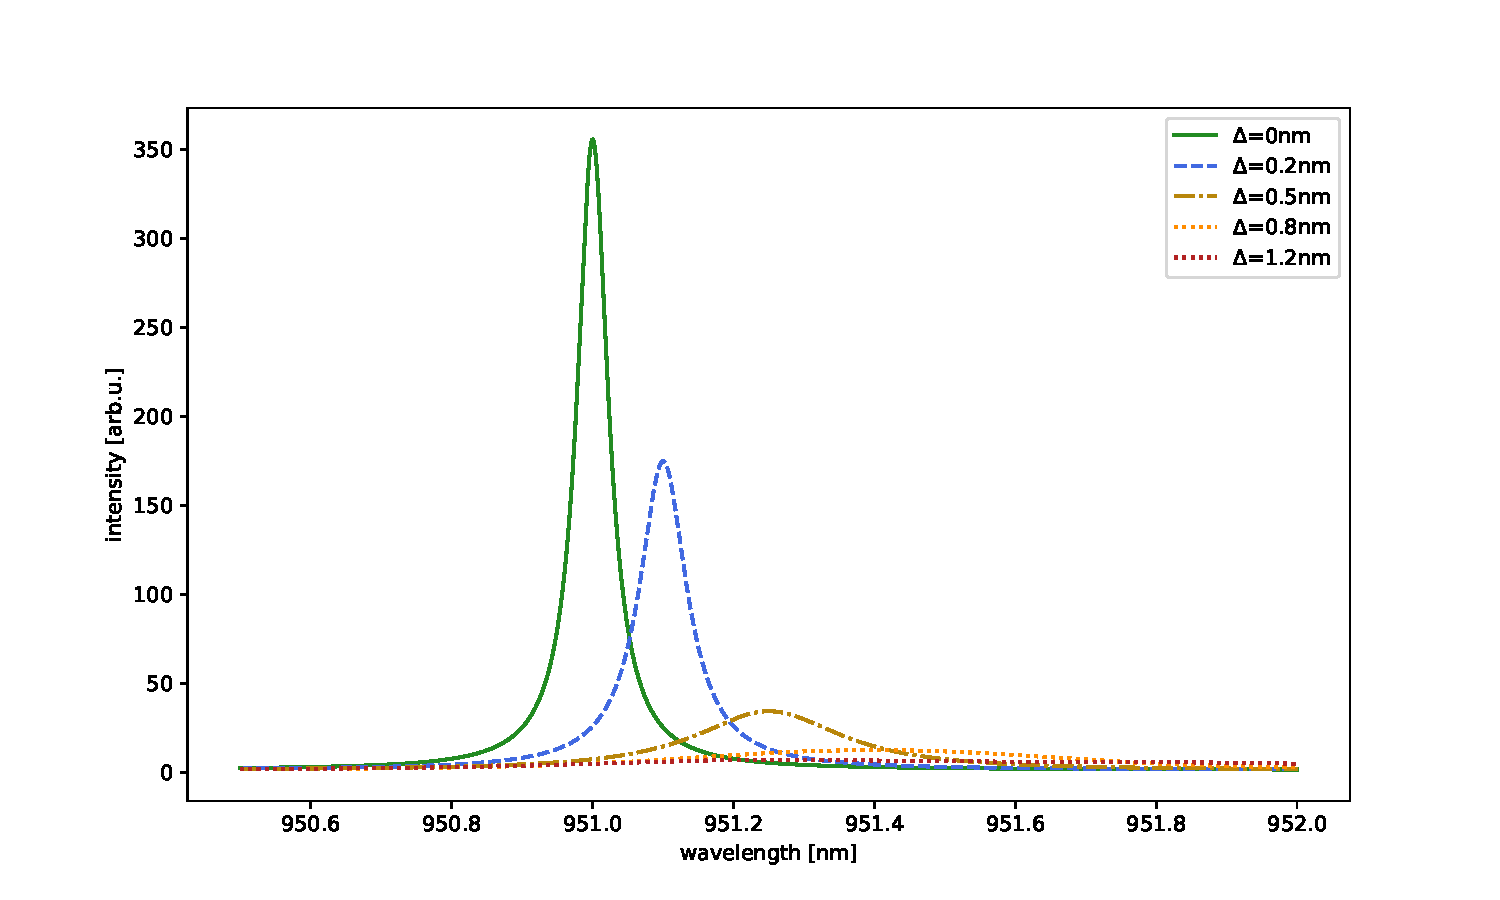
\includegraphics[width=\textwidth]{figures/detuning_scan_intracavity_double_fano_30um.pdf}
        \caption{Double Fano cavity intracavity spectra for different values of the spectral detuning $\Delta$.}
        \label{fig:intracavity_detuning_scan}
    \end{subfigure}
    \caption{}
    \label{fig:detuning_threshold_lossless}
\end{figure}

It is readily seen that with increasing detuning the peak shifts to the right, which is in itself a behavior which is trivial from eq. (\ref{eq:transmission_wavelength}). The linewidth is also seen to increase with larger detuning, and the peak eventually collapses when the overlap between the guided-mode resonance profiles of the two gratings becomes too small to sustain the Fano resonance. Figure \ref{fig:intracavity_detuning_scan} shows the intracavity spectra corresponding to the transmission spectra in figure \ref{fig:detuning_scan}, and provides valuable insight into the mode density inside the cavity for the different values of $\Delta$. It is clearly demonstrated by the two figures that the spectral overlap is a very crucial parameter of the double Fano cavity, and is paramount in describing the cavity's ability to sustain the Fano resonance modes. 

%% Write about the spacial detuning (should the order of the spectral and spacial detuning be reversed?)

\begin{figure}[h!]
    \centering
    \begin{subfigure}[b]{0.49\textwidth}
        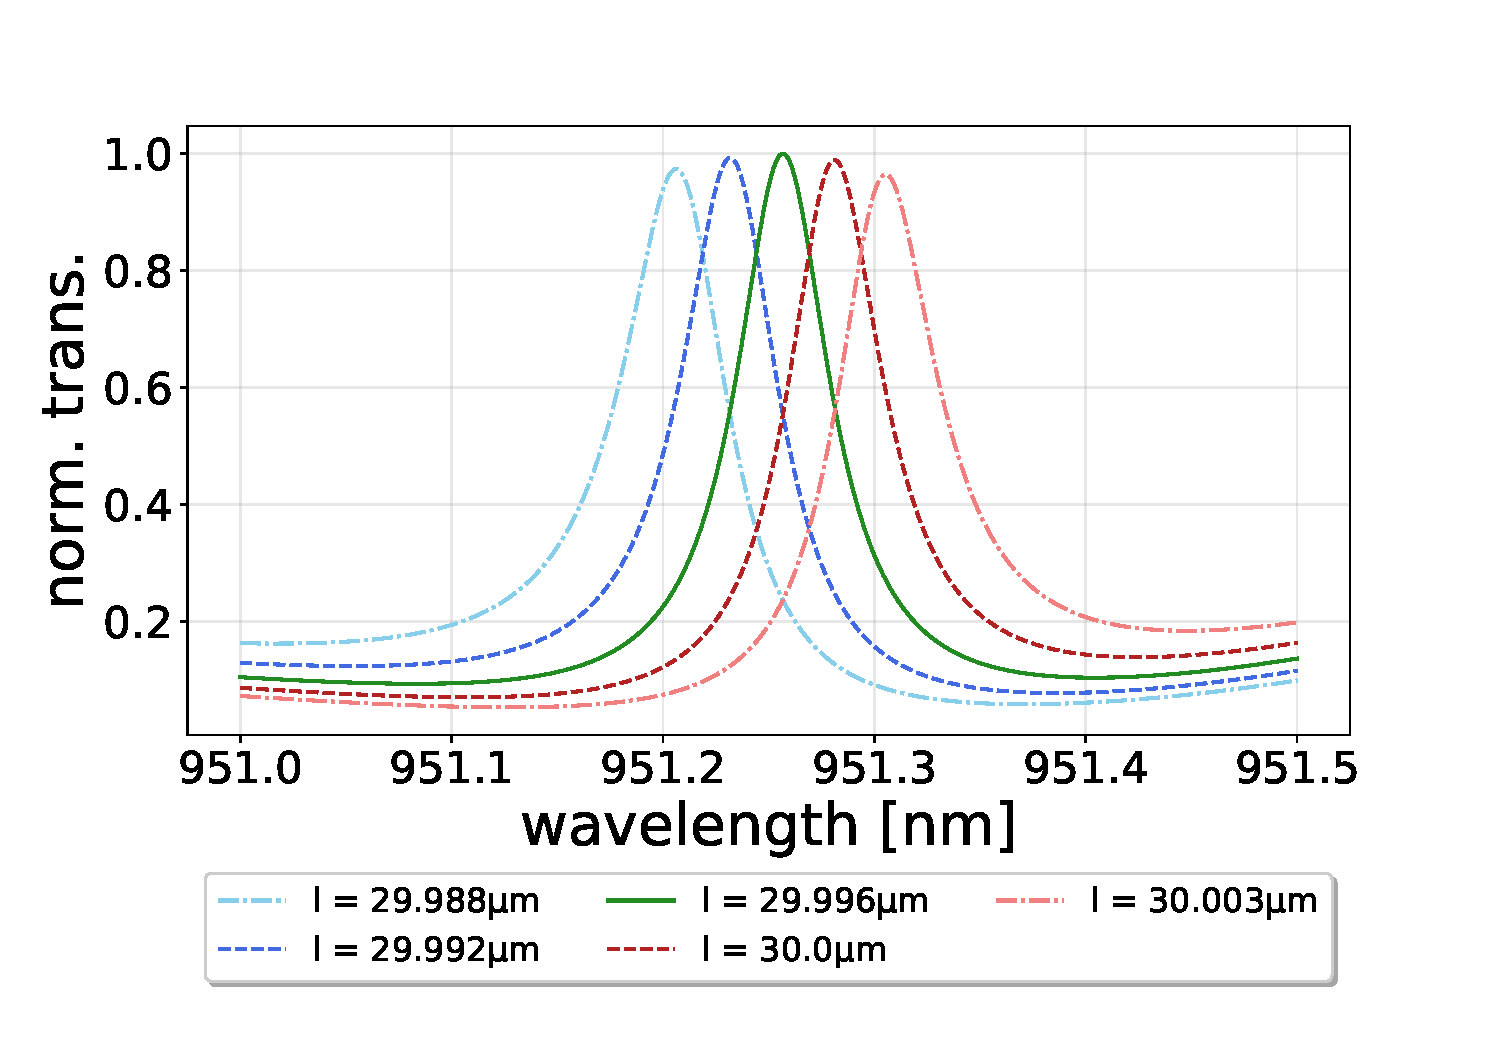
\includegraphics[width=\textwidth]{figures/small_detuning_length_scan_short.pdf}
        \caption{$\Delta = 0.1nm$}
        \label{fig:detuned_small_length_scan_long}
    \end{subfigure}
    \begin{subfigure}[b]{0.49\textwidth}
        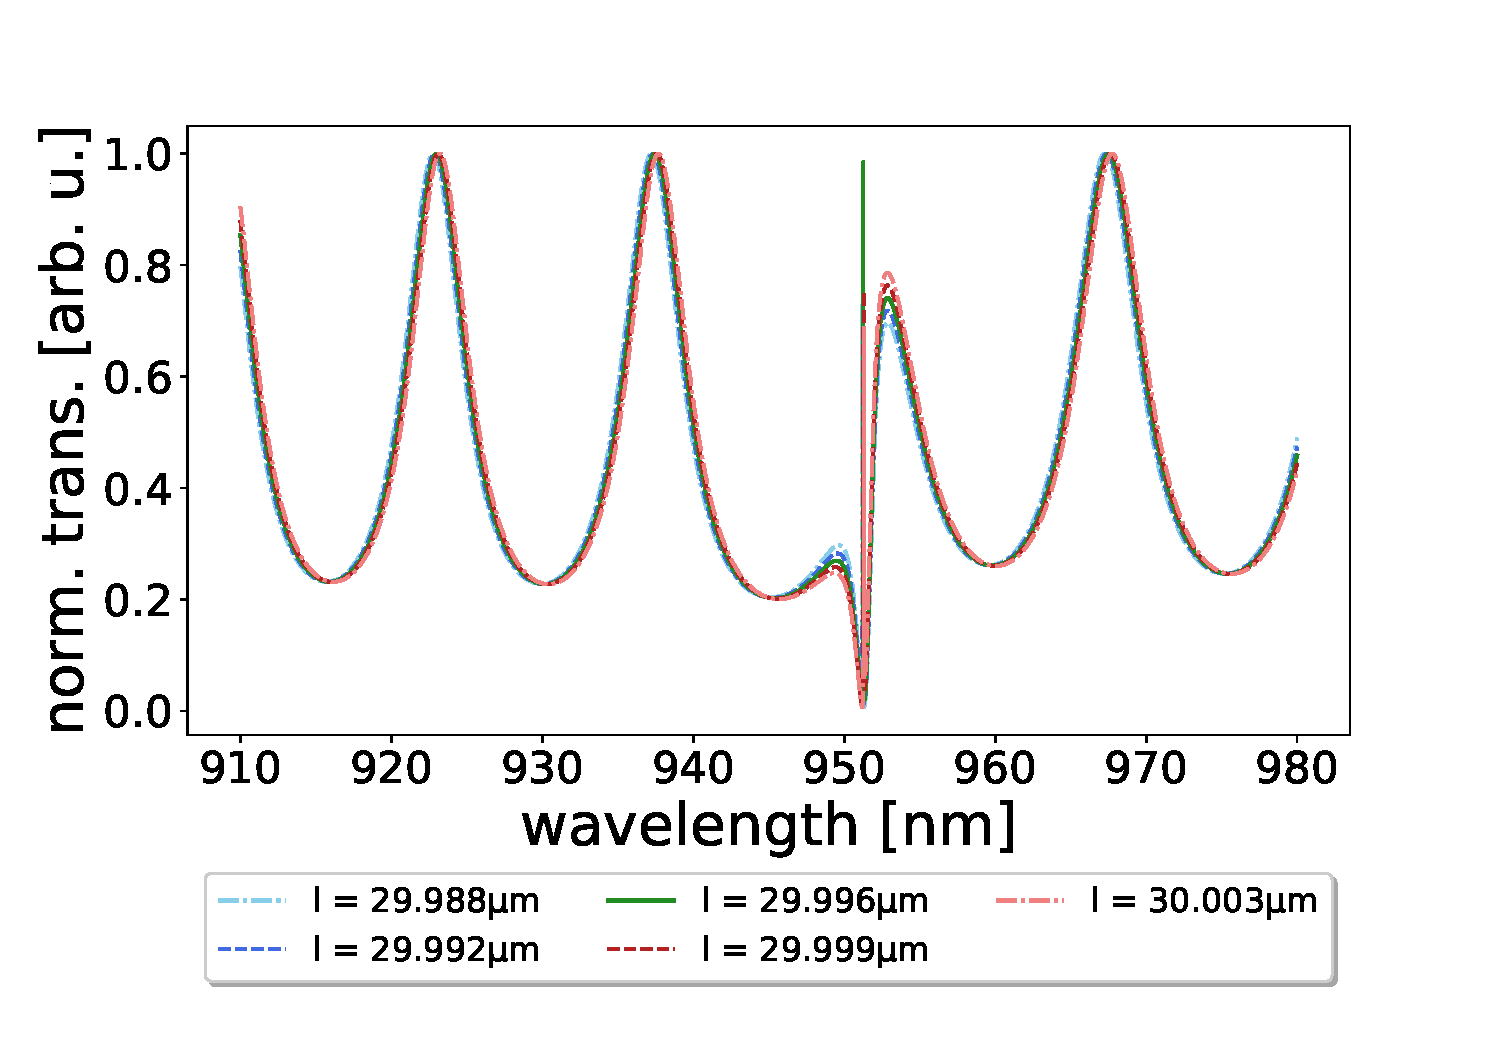
\includegraphics[width=\textwidth]{figures/small_detuning_length_scan_long.pdf}
        \caption{}
        \label{fig:detuned_small_length_scan_short}
    \end{subfigure}
    \caption{}
\end{figure}

\begin{figure}[h!]
    \centering
    \begin{subfigure}[b]{0.49\textwidth}
        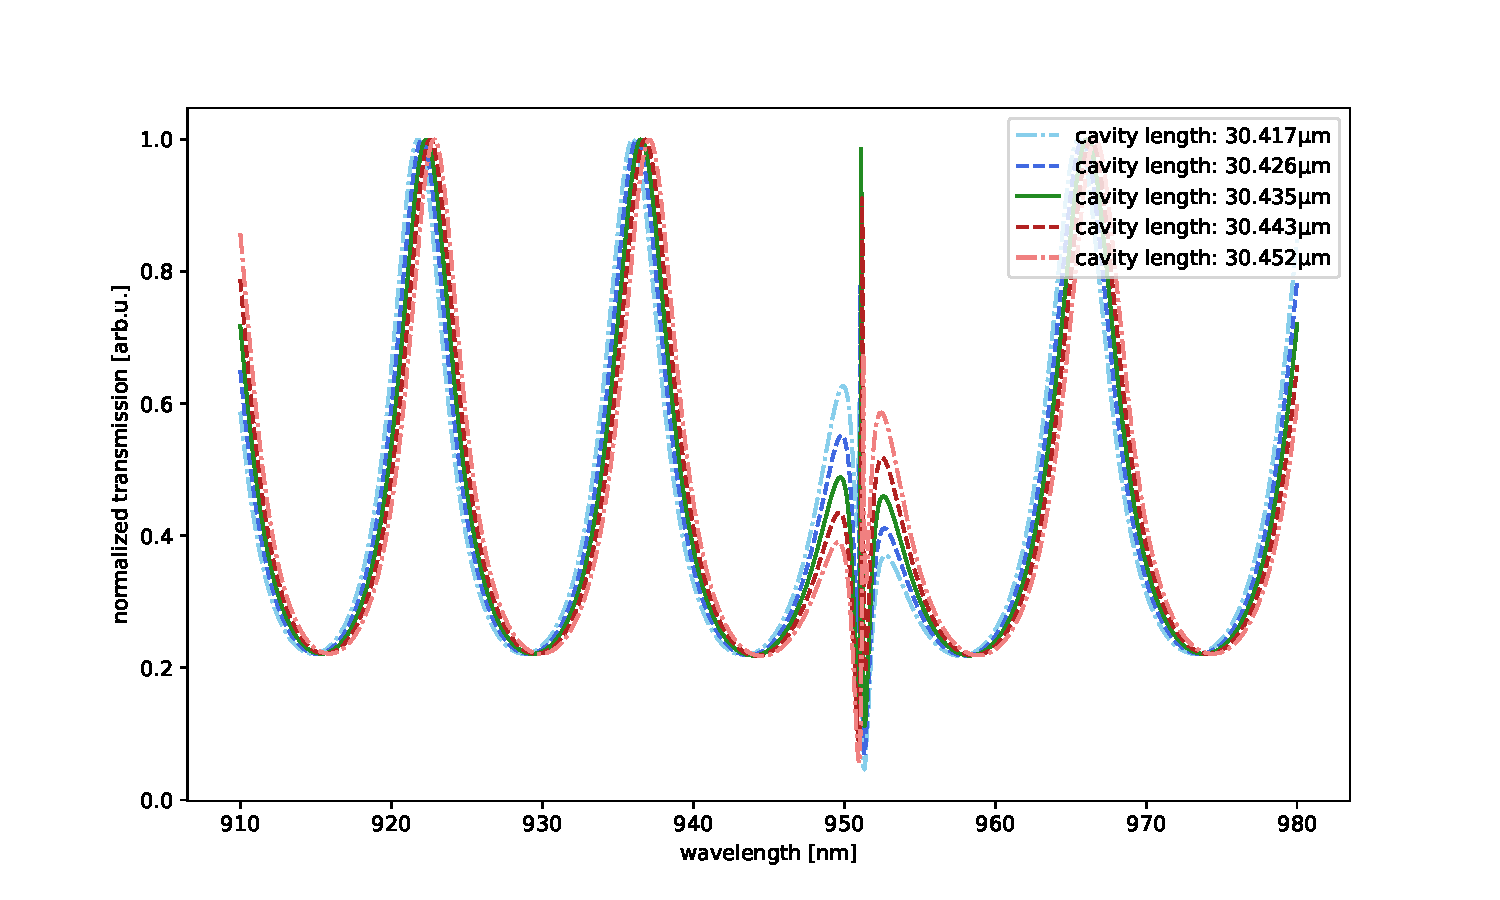
\includegraphics[width=\textwidth]{figures/detuned_length_scan_long.pdf}
        \caption{$\Delta = 0.3nm$}
        \label{fig:detuned_length_scan_long}
    \end{subfigure}
    \begin{subfigure}[b]{0.49\textwidth}
        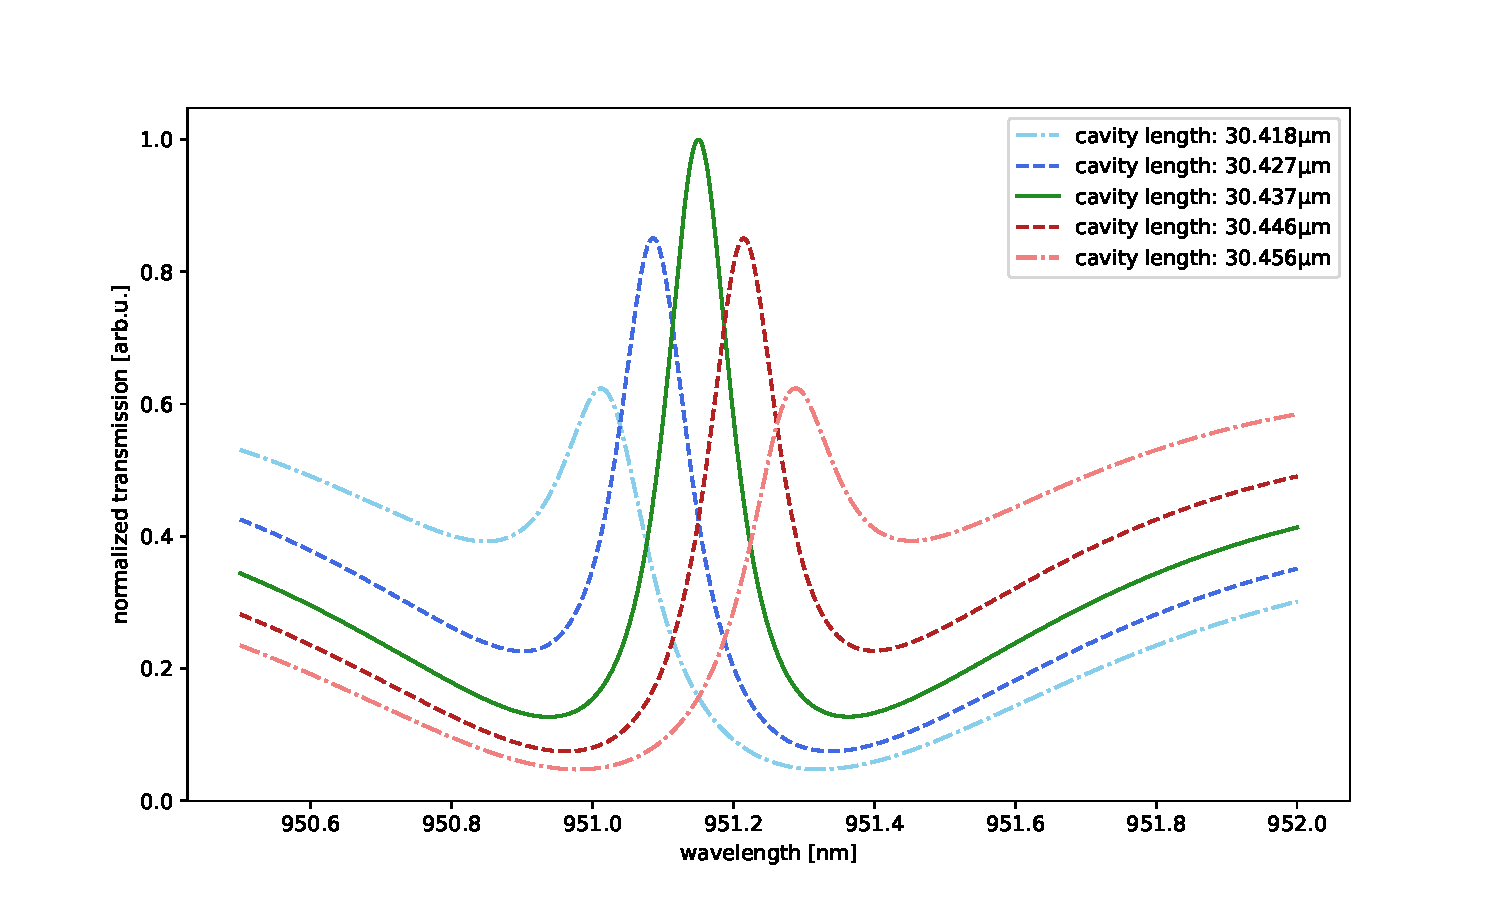
\includegraphics[width=\textwidth]{figures/detuned_length_scan_short.pdf}
        \caption{}
        \label{fig:detuned_length_scan_short}
    \end{subfigure}
    \caption{}
\end{figure}

\begin{figure}[h!]
    \centering
    \begin{subfigure}[b]{0.49\textwidth}
        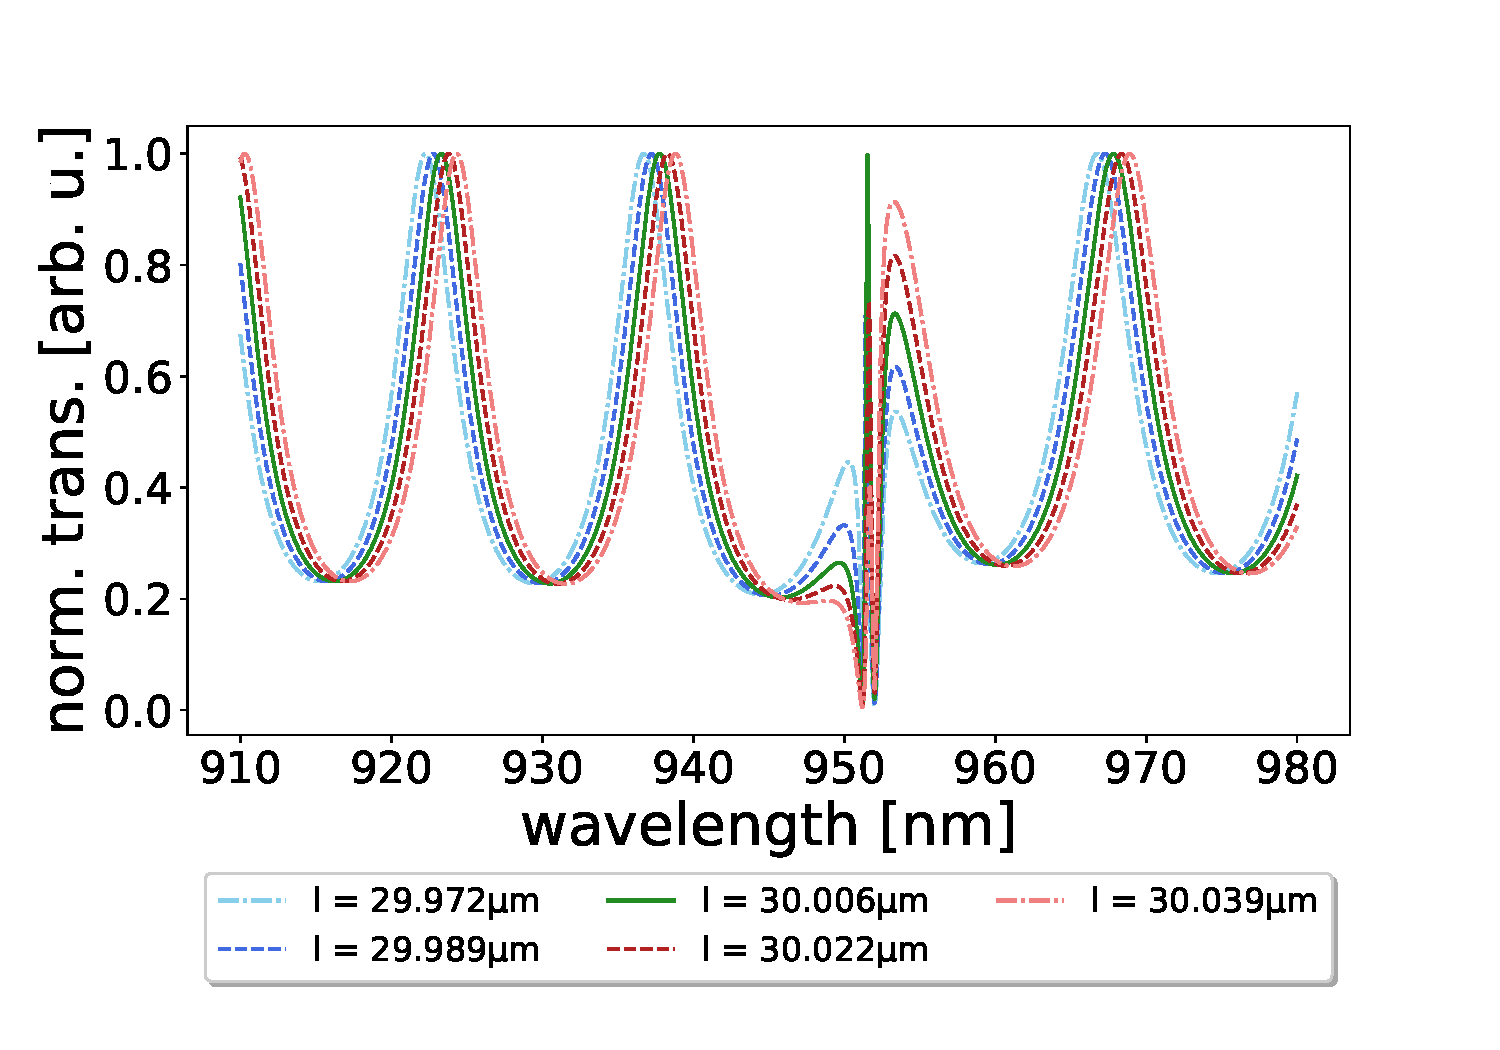
\includegraphics[width=\textwidth]{figures/large_detuning_length_scan_long.pdf}
        \caption{$\Delta = 0.8nm$}
        \label{fig:detuned_large_length_scan_long}
    \end{subfigure}
    \begin{subfigure}[b]{0.49\textwidth}
        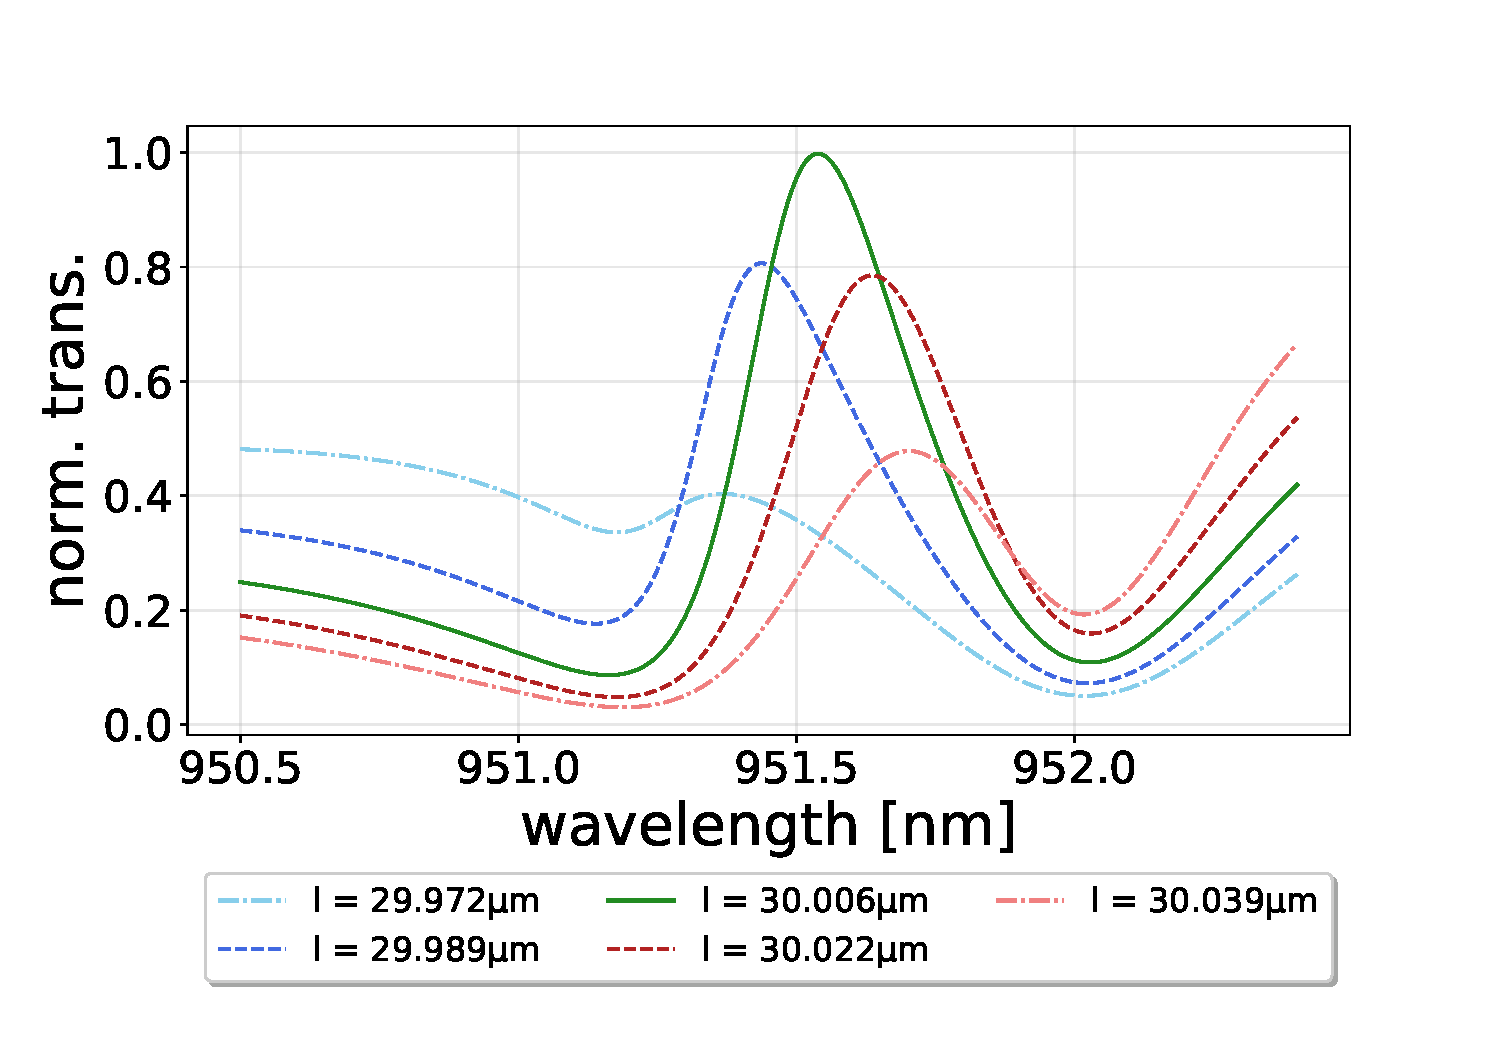
\includegraphics[width=\textwidth]{figures/large_detuning_length_scan_short.pdf}
        \caption{}
        \label{fig:detuned_large_length_scan_short}
    \end{subfigure}
    \caption{}
\end{figure}

\begin{figure}[h!]
    \centering
    \begin{subfigure}[c]{0.49\textwidth}
        \centering
        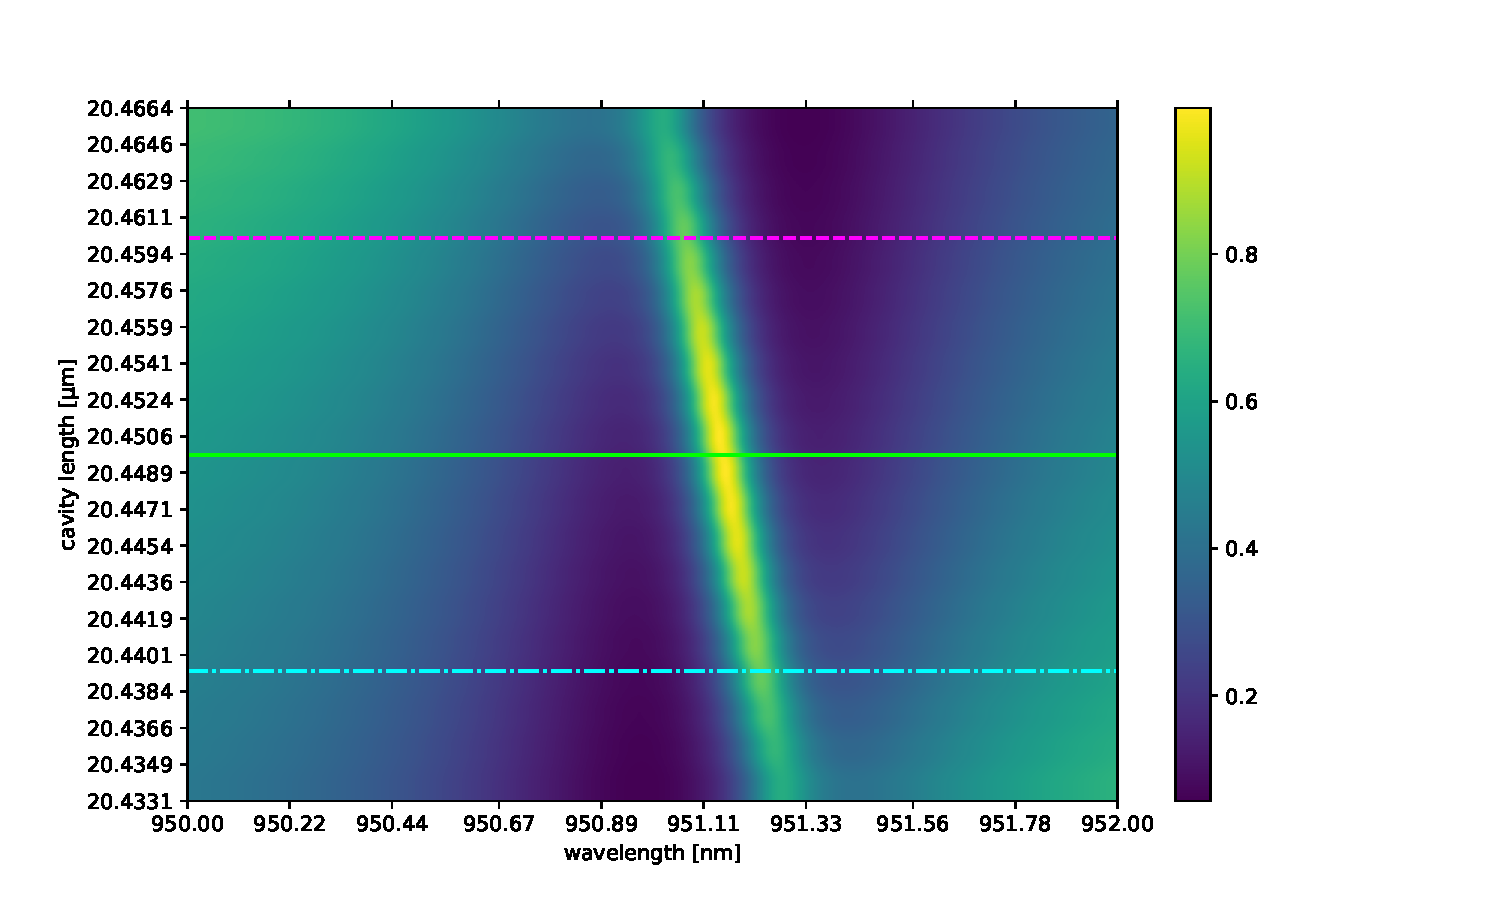
\includegraphics[width=\textwidth]{figures/cmap_with_slice_indicators1.pdf}
        \caption{cmap showing transmission as a function of wavelength for cavity lengths ranging $l_{g} \rightarrow l_{g}^{\prime}$ for $\Delta = 0.3nm$.}
    \end{subfigure}
    \begin{subfigure}[c]{0.49\textwidth}
        \centering
        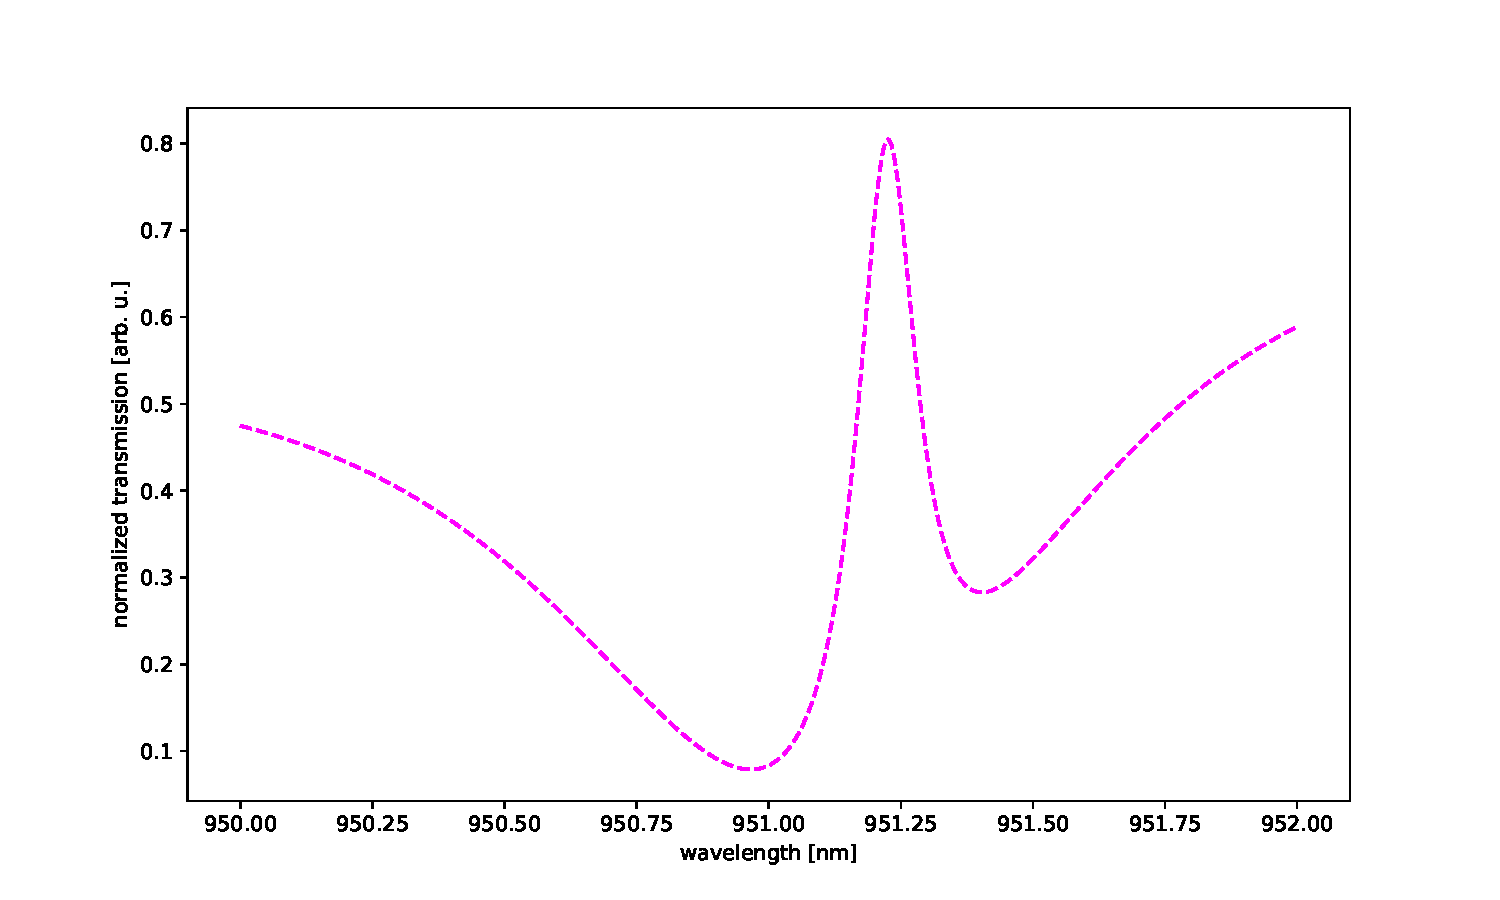
\includegraphics[width=0.49\textwidth]{figures/cmap_slice2.pdf}
        \newline
        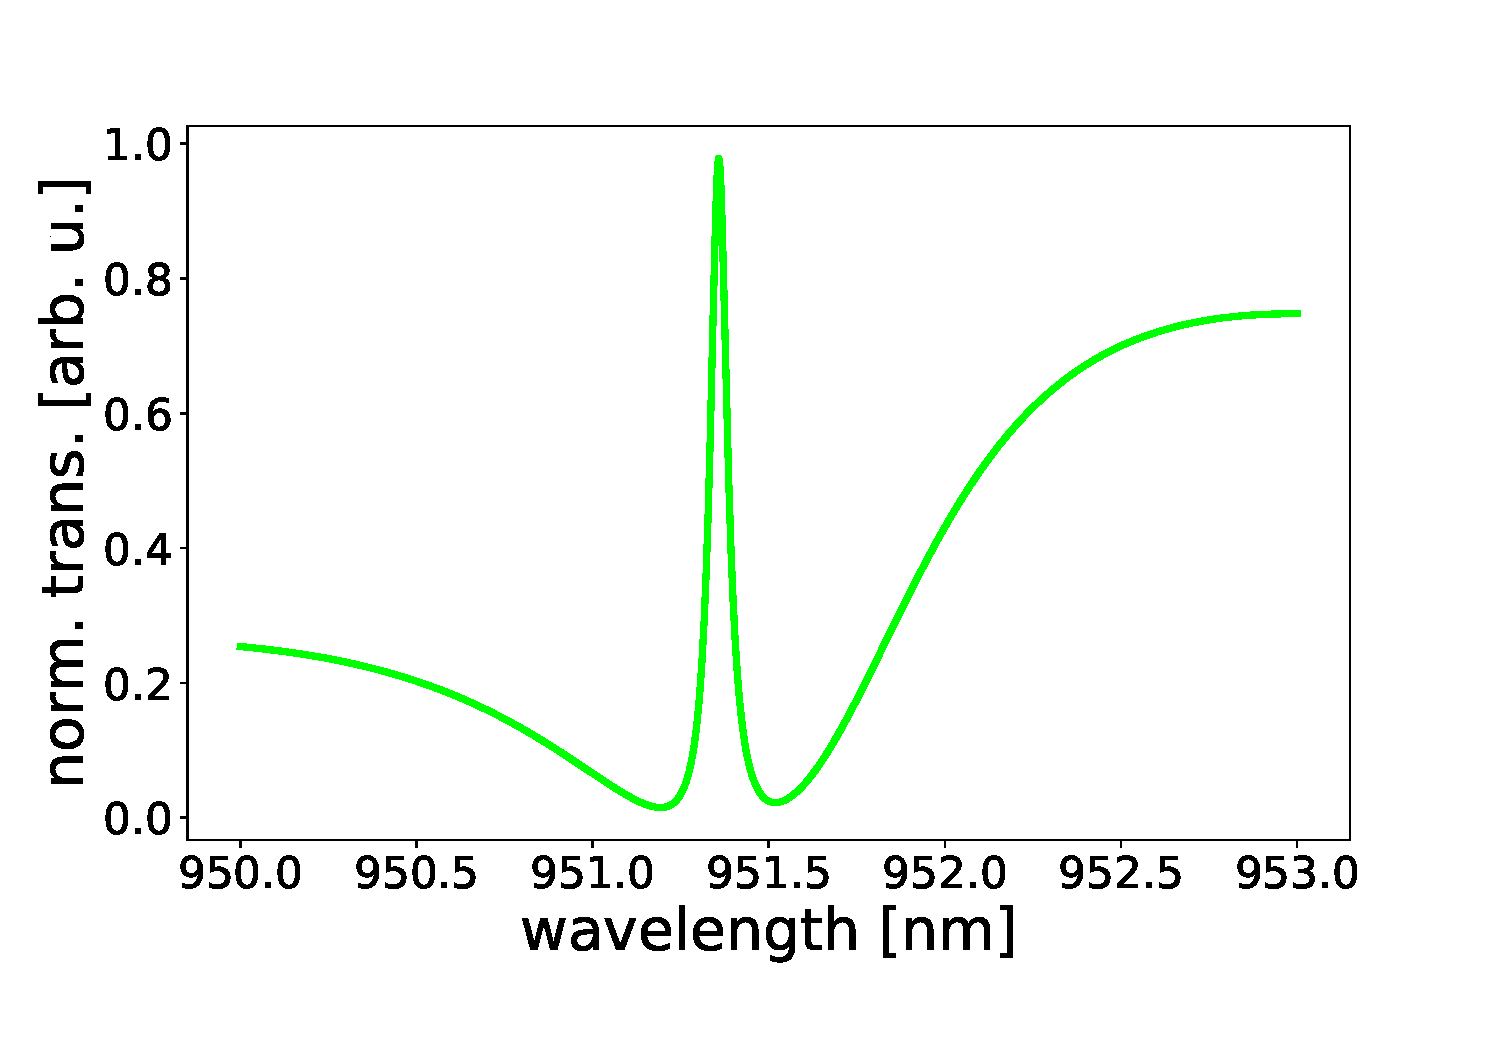
\includegraphics[width=0.49\textwidth]{figures/cmap_slice1.pdf}
        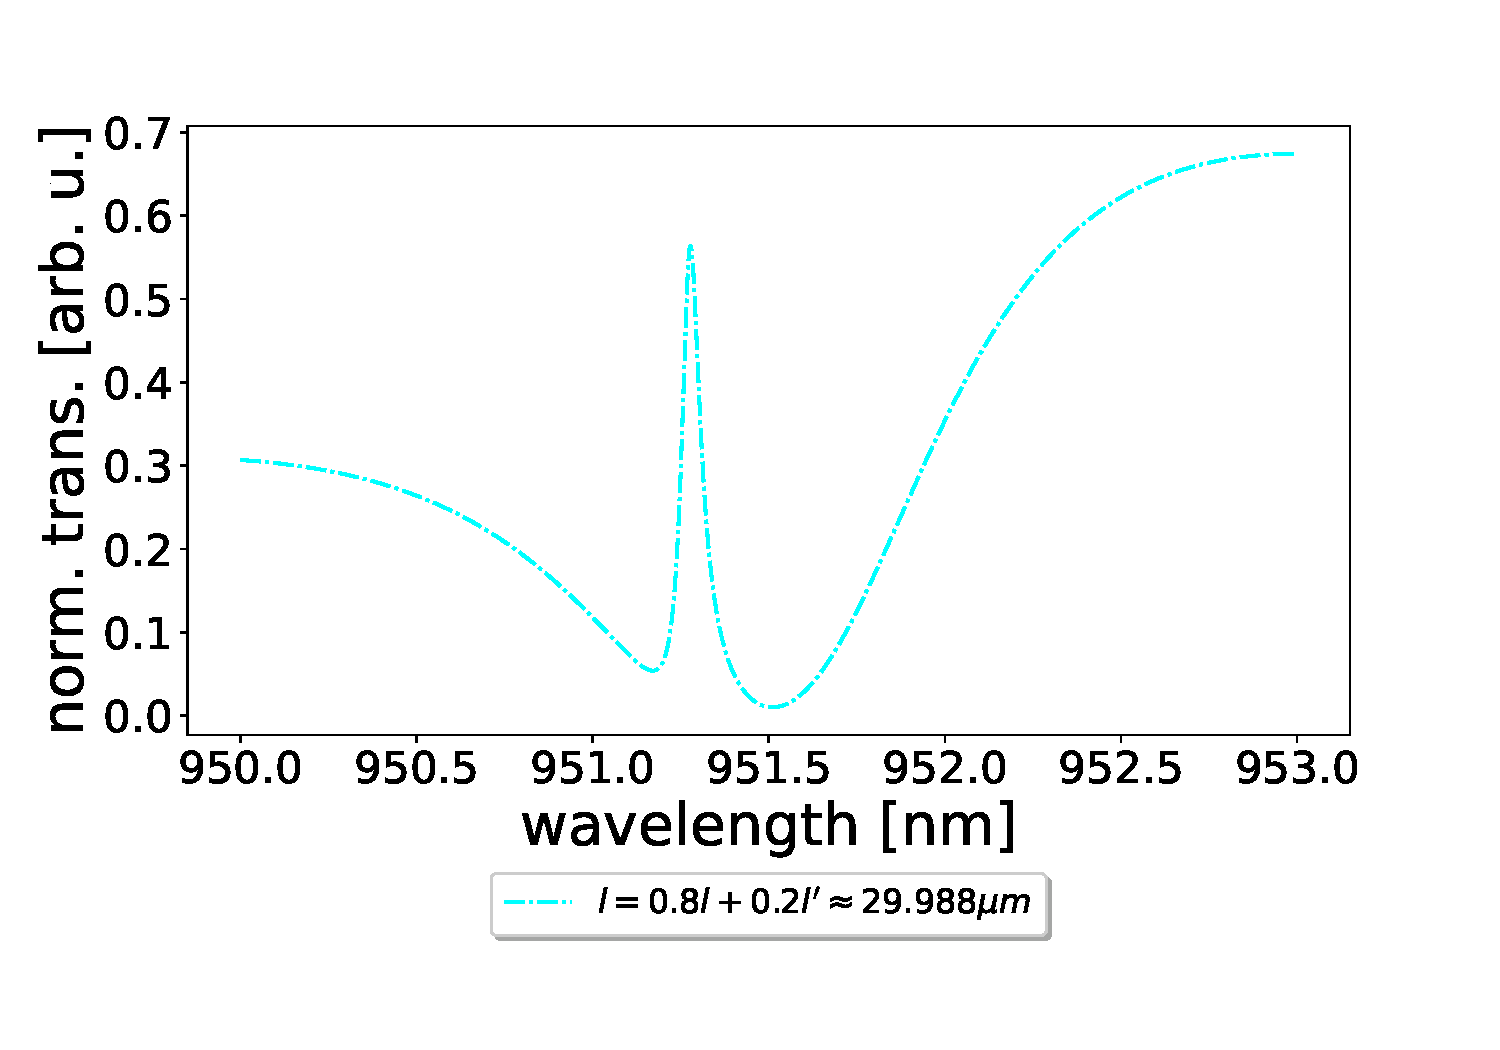
\includegraphics[width=0.49\textwidth]{figures/cmap_slice3.pdf}
        \caption{Slices of the cmap showing the optimal length and wavelength of double fano cavity (lossless). HWHMs -> Magenta = 71.3pm, cyan = 71.3pm and lime = 58.6pm.}
    \end{subfigure}
\end{figure}

\begin{figure}
    \centering
    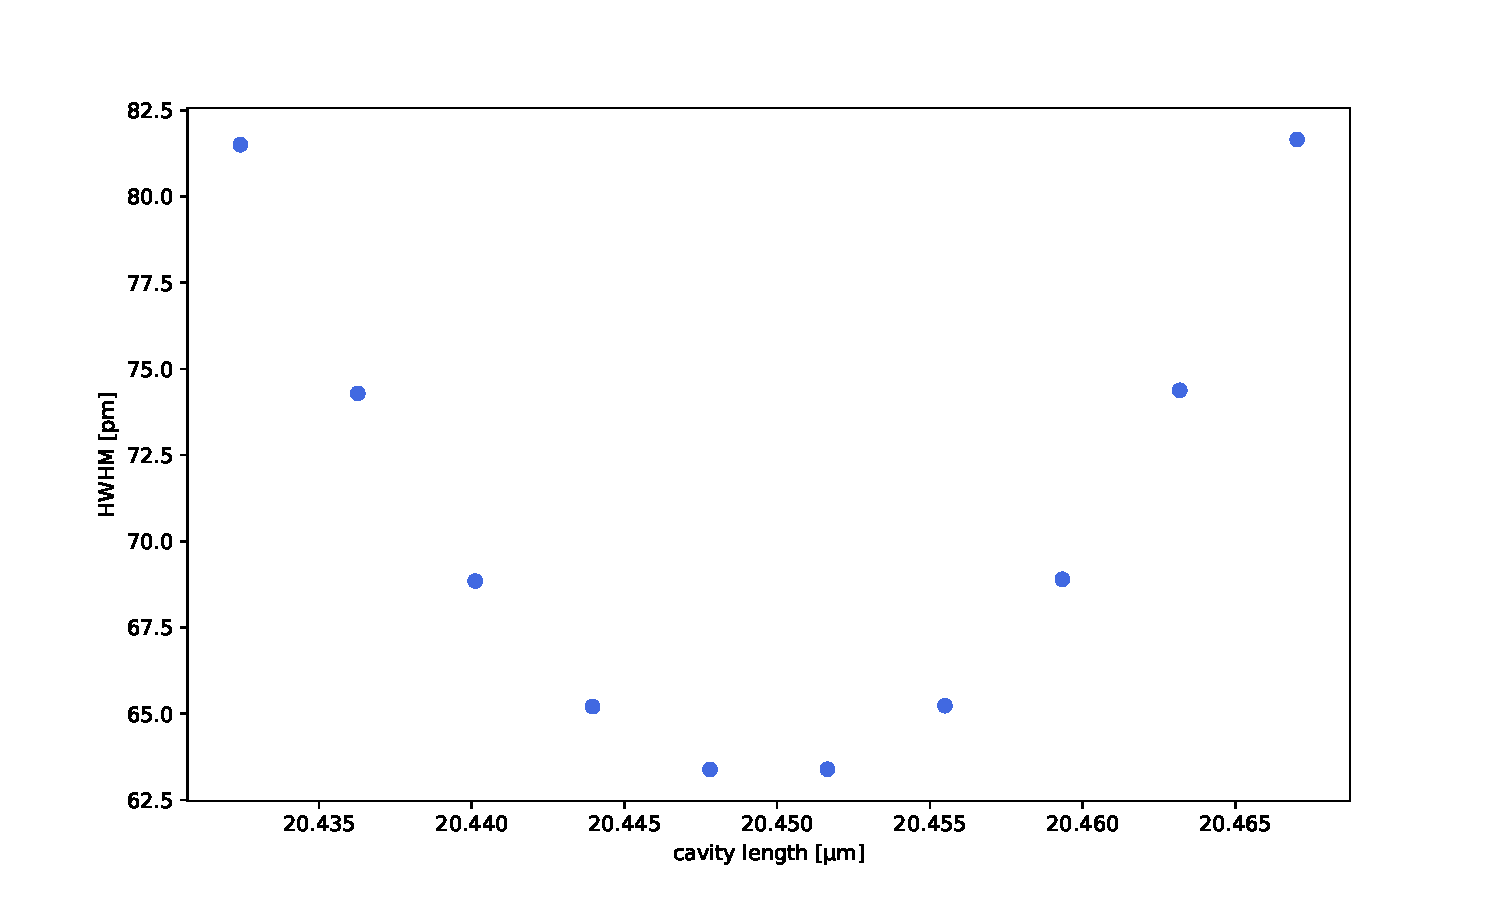
\includegraphics[width=0.5\textwidth]{figures/cmap_lw_vs_l_intracavity.pdf}
    \caption{intracavity linewidth as a function of cavity length (same cavity as depicted in cmap above.)}
\end{figure}

